\documentclass{tesis-usach}
% Opciones: propuesta

\usepackage{nameref}
\usepackage{booktabs}
\usepackage{adjustbox}
\usepackage{mathtools}
\DeclarePairedDelimiter{\ceil}{\lceil}{\rceil}

\begin{document}
\baselineskip 23pt
\frontmatter								% Utiliza numeración romana

% ### Cubierta de la tesis ###
\thispagestyle{empty}
\facultad{Facultad}
\departamento{Departamento}
\grado{Grado}

\titulo{Sistema escalable para la detecci\'on de necesidades en escenarios de cat\'astrofe natural}

\autor{Esteban Andrés Abarca Rubio}
\email{esteban.abarca@usach.cl}
\run{17.679.923-4}		% S\'olo necesario en propuesta
\telefono{997529097}		% S\'olo necesario en propuesta
\annoingreso{2010}

\fecha{Domingo}{15}{Mayo}{2016}

\profesorguia{Nicol\'as Hidalgo Castillo}
\profesorcoguia{Erika Rosas Olivos}

\ciudad{Santiago}
\pais{Chile}

\makecubierta


% ### Páginas preliminares de la tesis ###
\pagestyle{fancy}
\renewcommand{\headrulewidth}{0pt}		% Hace que no aparezca la línea horizontal superior al principio de estas páginas
\fancyhead[L]{}
\fancyhead[C]{}
\fancyhead[R]{}

{\setstretch{1.0}						% Interlineado en las páginas preliminares
\makecopyright							% Si es propuesta no se mostrará

\setcounter{page}{1} 
\resumenCastellano{

\textit{Twitter} es una red social que cuenta con millones de usuarios en todo el mundo y, en Chile, alcanza cerca de los 1.700.000 accesos diariamente. Sus usos van desde ser un \textit{microblog} personal hasta la entrega de información o comunicación entre pares. Es por ello que, en épocas de necesidad, como lo es el periodo inmediato luego de la ocurrencia de una catástrofe natural, las personas tienden a publicar sus experiencias dentro de éste servicio.


Teniendo en cuentra lo anterior es que se construyó un sistema, basado en el paradigma de procesamiento de \textit{streams}, capaz de recoger información de manera automática desde \textit{Twitter} — los denominados \textit{tweets} — y procesarlos a fin de detectar si es que un \textit{tweet} corresponde a uno en el que el usuario haga mención alguno de los tipos de necesidad que el sistema es capaz de detectar y, finalmente, hacer uso de la información implícita (contenido del \textit{tweet} o metadatos), para presentar la necesidad como un punto en un mapa geográfico del país, de modo que la información obtenida pueda ser tomada por las autoridades correspondientes para que, de esta forma, facilite el proceso de toma de desiciones en cuanto al envío de ayuda a una determinada área dadas las necesidades expresadas por la población. 

Para lograrlo se hizo uso de programación extrema en conjunto con la metodología KDD para construir una aplicación que haga uso de un clasificador de textos para la detección de necesidades, mediante los cuales se logra ubicar y clasificar correctamente datos obtenidos del terremoto de Concepción ocurrido el 27 de febrero del año 2010. Además se prueba la efectividad del operador detector de ubicación para suplir la carencia de datos de geolocalización en los metadatos de \textit{Twitter}.

Este trabajo se enmarca en el proyecto FONDEF IDeA (Dos etapas) código ID15I10560 en el que participa un equipo de investigación de la universidad.


\vspace*{0.5cm}
\KeywordsES{Programación extrema; KDD; Clasficador; \textit{Twitter}; Detección de necesidades; Geolocalización; \textit{Stream processing}; Clasificador de texto; Redes sociales; Herramienta de apoyo a desastres}
}

\newpage

\resumenIngles{
\textit{Twitter} is a social network that already has millions of users worldwide and, in Chile, reach about of 1.7 millions of accesses daily. Its uses range from being a personal microblog up to information delivery and comunication between peers. It's because of this that in emergencies, such as the inmediate period after a natural catastrophe, people tends to post their experiences on this service.

With this in mind is that is built a system, based on stream processing paradigm, that it's able to get, automatically, information from \textit{Twitter} — as \textit{tweets} — and process it to detect if a user's \textit{tweet} mentions one of the needs that the system can handle and, finally, use the implicit information in the tweet (metadata) and render the need as a geographical position in country's map, thus authority can use the given information and ease the desition making process of sending help to affected areas with the information given by the population.

To achieve these statements previously exposed extreme programming has been used in conjunction with KDD in order to build a text's classifier to detect people's needs. With these two methods was possible to classify and place correctly the data obtained from Concepción's earthquake at February the 27, 2010. It was proved the effectiveness of the proposed location recognizer created to supply the lack of geolocalization data in Twitter's metadata.

This project is within the FONDEF IDeA (Two stages), code: ID15I10560, where a University's research team is working on.

\vspace*{0.5cm}
\KeywordsEN{Extreme programming; KDD; Classifier; Twitter; Detect people's Need; Geolocalization; Stream processing; Text's classification; Social networks; Post-disaster support tool}
}


% ### Dedicatoria y agredecimientos de la tesis ###
\dedicatoria{
Dedicado a...
}
		% En caso de no querer agregarlos, comente esta línea
\begin{agradecimiento}
Agradezco a
\end{agradecimiento}

% ### Índices ###
\tableofcontents							%% Tabla de contenido

\listoftables							%% Indice de tablas
\listoffigures							%% Indice de figuras
\listofalgorithms						%% Indice de algoritmos
\AtBeginEnvironment{algorithmic}{\setstretch{1.5}} % Interlineado de los algoritmos
} % end \setstretch{1.0}

% ### Cuerpo de la tesis ###
\mainmatter								% Reinicia el contador de páginas para partir de 1 y usando números arábicos.

% ### Capítulos de la tesis ###
\chapter{Introducción}
\label{cap:introduccion}

\section{Antecedentes y motivación}
\label{intro:motivacion}

Los desastres naturales en Chile han sido frecuentes en los últimos años. Sólo por mencionar algunos de los más recientes: la erupción del volcán Chaitén (Mayo, 2008), el terremoto en Tocopilla (Noviembre, 2007), el terremoto en Concepción (2010), el incendio de las Torres del Paine (Diciembre, 2011), el incendio en Valparaíso (Abril, 2014), la erupción del volcán Villarrica (Marzo, 2015), los aluviones en el norte (Marzo, 2015), entre otros. Dependiendo de las características de la emergencia, surgen en la población diversos tipos de necesidades: alimentos, agua, luz eléctrica, refugio, rescate o comunicación. Muchas veces éstas pueden no ser detectadas por las autoridades; al menos, no de forma expedita, lo que resulta perjudicial para las personas que intentan sobrellevar, de la mejor manera posible, la crisis cuando se ve involucrada una necesidad básica, como la falta de agua, donde la vida de los afectados puede verse comprometida. El problema anteriormente descrito, no es sólo para las autoridades; \cite{ChatoSurvey}, señalan que el comportamiento humano ante crisis como éstas, no es quedarse esperando por ayuda o huir en pánico, sino de intentar tomar decisiones rápidas en base a la información que conocen. Esto quiere decir que existe gente dispuesta a ayudar, aun siendo ellos mismos los afectados; pero no siempre disponen de la información necesaria para saber hacia dónde apuntar sus esfuerzos. Será útil, dado todo lo anterior, tener algún medio que concentre las necesidades que pueda tener una población dentro del país, para acudir en su auxilio posterior a la ocurrencia de una emergencia catastrófica, como las mencionadas anteriormente.

Los académicos del proyecto FONDEF IDeA de la Universidad de Santiago de Chile, están trabajando en el desarrollo de una plataforma de procesamiento de flujo de datos generados en contextos de desastres; se busca proveer la infraestructura necesaria para la generación de herramientas capaces de apoyar la toma de decisiones en escenarios de desastres. Esta plataforma hace uso de la información generada por los usuarios en redes sociales como fuente de datos. Para realizar la prueba de concepto de la plataforma se planea desarrollar tres aplicaciones base, orientadas a facilitar la coordinación de voluntarios, detección de necesidades y difusión de información de interés.

En particular, para este trabajo, se ataca el problema de la detección de necesidades de la población y servir de apoyo para la construcción de la plataforma de \textit{streaming}, en relación a qué operadores se han de construir y cómo ha de estructurarse el sistema para operar sobre datos nacionales.

\section{Descripción del problema}
\label{intro:problema}

El problema que aborda esta memoria, es el hacer uso de la información generada por la población por medio de \textit{Twitter} para que, en caso de alguna emergencia de carácter nacional, pueda prestarse apoyo en tiempo real a las autoridades encargadas de la toma de decisiones; por ejemplo, dándoles a conocer en qué lugar exactamente se requiere asistir a la población con un determinado tipo de ayuda, según la necesidad que se presente. ¿Cómo detectar y localizar en tiempo real las necesidades expresadas por la población en redes sociales basadas en texto de manera de entregar generar una nueva fuente de datos para mejorar la toma de decisiones?

\section{Solución propuesta}
\label{intro:solucion}

Se propone un sistema capaz de recoger y analizar de manera automática los eventos generados en la red social \textit{Twitter} en tiempo real, de manera que, al ocurrir un escenario de desastre, determine si la publicación expresa una necesidad y, en caso de que así sea, determine su posición geográfica. 

La solución propuesta consta de dos partes: Por una lado la plataforma y lógica de procesamiento capaz de realizar la labor antes mencionada y, por otro, la visualización de estos datos.

Dado que se utiliza \textit{Twitter} para obtener los datos de entrada, los cuales llegan mediante el \textit{stream} producido por la API de esta red social, la plataforma de procesamiento consiste en un sistema de procesamiento de \textit{streams}, construido utilizando el sistema de computación distribuida de Apache, \textit{Storm}, el cual basa su procesamiento en transformar el problema en un grafo donde cada nodo aporta realizando sólo una tarea, pero que pueden existir múltiples instancias de aquel nodo y éstos pueden estar en diferentes máquinas. Así, internamente, la plataforma está compuesta de operadores que discriminan cuándo evento debe ser entregado a la aplicación de visualización para ser mostradas al usuario. Uno de estos operadores permitirá realizar la categorización del texto de entrada por medio un un clasificador bayesiano.

\section{Objetivos y alcance del proyecto}
\label{intro:objetivos}

\subsection{Objetivo general}
	Construir un sistema escalable para la detección de necesidades de la población en tiempo real, para escenarios de desastre natural haciendo uso de \textit{Twitter}.

\subsection{Objetivos específicos}
\begin{enumerate}
\item	Implementar un método encargado de la recolección de tweets generados dentro del territorio nacional haciendo uso de la API pública de Twitter.
\item	Especificar la taxonomía de las necesidades detectadas.
\item	Diseñar e implementar el clasificador de necesidades.
\item	Definir los elementos de procesamiento para la construcción del sistema capaz de trabajar los datos obtenidos a gran escala.
\item	Implementar una arquitectura escalable que soporte la aplicación.
\item	Evaluar la aplicación bajo condiciones de alto tráfico, como es el caso de una emergencia nacional.
\end{enumerate}

\subsection{Alcances}
\label{subsec:alcances}

Se utilizan las publicaciones de \textit{Twitter} para llevar a cabo el procesamiento de la información y no se considera, en el marco de este trabajo, el uso de una red social alternativa, no porque no sea posible, sino que con el motivo de acotar el problema.

Las necesidades que la aplicación detecta no son una lista exhaustiva de las posibles existentes, sino de un subconjunto que se ha considerado más importante en el equipo de trabajo del proyecto. De esta forma se logra acotar el problema reduciendo la cantidad de categorías y permitir una mayor precisión en la clasificación, entendiendo la precisión como la relación de elementos clasificados correctamente sobre el total.

Se considera, para la construcción del clasificador, un subconjunto de un \textit{dataset} compuesto de cuatro millones de \textit{tweets} recogidos durante y posteriormente al terremoto en Concepción el 27 de Febrero del 2010. Éste conjunto de datos ha de ser limpiado previamente pues contiene \textit{tweets} en idiomas diferentes al idioma objetivo de este trabajo.

El sistema sólo trabaja en la detección con \textit{tweets} que estén en español.

La validación se realiza a partir de \textit{datasets} con \textit{tweets} reales, sin embargo los flujos generados son sintéticos y no obtenidos de manera online desde \textit{Twitter}.

\section{Metodologías y herramientas utilizadas}
\label{intro:metodologia}

\subsection{Metodología}
\label{subsec:MetodologiaDetalle}

Para la realización de este trabajo se utilizan dos metodologías, la primera está enfocada a la búsqueda de información en bases de datos para realizar la construcción del clasificador de texto, mientras que la segunda, una metodología de desarrollo de aplicaciones ágil está enfocada en la construcción en sí de las aplicaciones, tanto de la plataforma de procesamiento como de la aplicación de visualización. Ambas son definidas a continuación.

\subsubsection*{Programación Extrema}
\label{subsubsec:XP}

La Programación Extrema (\textit{Extreme Programming}, XP desde ahora en adelante), comenzó como un proyecto el 6 de Marzo de 1996. Es uno de los procesos ágiles más populares y ha sido probado exitosamente en compañias e industrias de todos los tamaños. \cite{XP}.

Su éxito se debe a que hace especial hincapié en la satisfacción del cliente por sobre la entrega de todo lo el software posible.

Aporta cinco formas escenciales para mejorar el proceso de desarrollo de software: comunicación, simplicidad, retroalimentación, respeto y coraje. Se busca en establecer una estrecha comunicación entre el equipo de desarrollo y el cliente apuntanto, paralelamente, a evitar el sobre-diseño y obtener retroalimentación de modo que los cambios puedan realizarse lo antes posible. 

La metodología implementa unas simples reglas de trabajo, las que se dividen en cinco grandes áreas las que se detallarán a continuación.

\begin{enumerate}
\item Planeación:
	\begin{itemize}
	\item Se escriben Historias de usuario. 
	\item Se crea un plan de \textit{releases}.
	\item Se planifican liberaciones pequeñas y frecuentes.
	\item Se divide el proyecto en iteraciones.
	\item Al comienzo de cada iteración se planea cómo será.
	\end{itemize}
\item Manejo:
	\begin{itemize}
	\item Se le da al equipo una área de trabajo.
	\item Se realizan reunione del tipo \textit{stand up meeting} a díario.
	\item Se mide la velocidad del proyecto. 
	\item Se mueven a las personas de sus puestos (para que todo el equipo pueda trabajar en todo).
	\item Se solucionan problemas que instroduzcan quiebres en la metodología.
	\end{itemize}
\item Diseño:
	\begin{itemize}
	\item Simplicidad. El mejor diseño es el más simple.
	\item Se crean \textit{spikes} para reducir el riesgo.
	\item No se agregan funcionalidades antes de tiempo.
	\item Hacer uso de técnicas de \textit{refactoring}, cada vez que sea posible.
	\end{itemize}
\item Implementación:
	\begin{itemize}
	\item El cliente siempre está disponible. 
	\item El código debe ser escrito bajo estándares. 
	\item Se hace uso de \textit{Test Driven Development }(TDD).
	\item Todo el código debe hacerse haciendo uso de \textit{pair programming}.
	\item Sólo una pareja integra código a la vez.
	\item Integración a menudo.
	\item Se cuenta con un equipo dedicado a la integración.
	\item El código es de todos.
	\end{itemize}
\item Prueba:
	\begin{itemize}
	\item Todo el código debe tener pruebas unitarias.
	\item Todas las pruebas deben ser pasadas antes de una liberación.
	\item Cuando se encuentra un \textit{bug}, se crean pruebas.
	\item Los \textit{test} de aceptación se corren a menudo y sus resultados son publicados.
	\end{itemize}
\end{enumerate}

Éstas reglas por sí solas pueden carecer de sentido, pero se apoyan en los \textbf{valores} que la metodología quiere entregar y que fueron mencionadas anteriormente, pero ahora son detalladas:

\begin{itemize}
\item Simplicidad: Se hace lo que se solicitó, pero no más. Ésto maximiza el valor entregado dado una fecha límite. Nuestras metas se alcanzan por medio de pequeños pasos para mitigar errores tan pronto ocurran. Se crea algo de lo que se esté orgullosos y lo se mantiene en el tiempo a costos razonables.
\item Comunicación: Todos somos partes de un equipo y nos comunicamos cara a cara a diario. Se trabaja juntos en todo: desde la toma de requerimientos hasta la implementación. Se crea la mejor solución posible al problema.
\item Retroalimentación: Cada iteración es completada seriamente entregando \textit{software} funcional. Mostraremos nuestro \textit{software} a menudo y prontamente para luego escuchar y aplicar los cambios solicitados. Se habla de nuestro proyecto y se adapta nuestro proceso a el, no al revéz.
\item Respeto: Todos dan y reciben el respeto que merecen como miembros del equipo. Todos contribuyen con valor así sea simple entusiasmo. Los desarrolladores respetan la experiencia del cliente y viceversa. 
\item Coraje: Se dice la verdad sobre el progreso y nuestras estimaciones. No se documentan excusas por si se falla, pues se planea tener éxito. No tenemos porque no trabajamos solos. Nos adaptaremos a los cambio cuando ocurran.
\end{itemize}

El proceso de XP puede puede ser apreciado en la Figura \ref{fig:procesoXP}.

\begin{figure}[H]
	\centering
	\captionsetup{justification=centering}
	\includegraphics[scale=0.6]{images/flowChartXP.png}
	\caption[Diagrama de flujo de Programación Extrema.]{Diagrama de flujo de Programación Extrema.\\Fuente: \cite{XP}}
	\label{fig:procesoXP}
\end{figure}

\subsubsection*{\textit{Knowledge Discovery in Databases} (KDD)}
\label{subsubsec:kdd}

Metodología de trabajo para la búsqueda de información en bases de datos, es definida por \cite{KDDFayyad} como "el proceso no trivial de identificar patrones válidos, nuevos, potencialmente útiles y en ultima instancia comprensible en los datos", surge de la necesidad de manejar grandes volúmenes de datos e involucra simultaneamente varias disciplinas de investigación tales como el aprendizaje automático, la estadística, inteligencia artificial, sistemas de gestión de bases de datos, sistemas de apoyo a la toma de decisiones, entre otras.

Si bien puede variar el usuario, quien es aquel que determina el domino de la aplicación, es decir, cómo se utilizan los datos, el proceso generalmente considera las siguientes etapas:

\begin{enumerate}
\item Selección de datos: Consiste en buscar el objetivo y las herramientas del proceso de minería, identificando los datos que han de ser extraídos, buscando atributos apropiados de entrada y la información de salida para representar la tarea. Esto quiere decir, primero se debe tener en cuenta lo que se sabe, lo que se quiere obtener y cuáles son los datos que nos facilitarán esa información para poder llegar a nuestra meta, antes de comenzar el proceso como tal.
\item Limpieza de datos: En este paso se limpian los atributos sucios, incluyendo datos incompletos, el ruido y datos inconsistentes. Estos datos sucios, en algunos casos, deben ser eliminados, pues pueden contribuir a un análisis inexacto y resultados incorrectos.
\item Integración de datos: Combina datos de múltiples procedencias incluyendo múltiples bases de datos, que pueden tener diferentes contenidos y formatos.
\item Transformación de datos: Consiste en modificaciones sintácticas llevadas a cabo sobre los datos sin que suponga un cambio en la técnica de minería aplicada. Tiene dos caras, por un lado existen ventajas en el sentido de mejorar la interpretación de las reglas descubiertas y reduce el tiempo de ejecución, por el otro puede llevar a la pérdida de información.
\item Reducción de datos: Reducción del tamaño de los datos, encontrando características más significativas dependiendo del objetivo del proceso.
\item Minería de datos: Consiste en la búsqueda de patrones de interés que puedan expresarse como un modelo o dependencia de los datos. Se ha de de especificar un criterio de preferencia para seleccionar un modelo de un conjunto de posibles modelos. Además se ha de especificar la estrategia de búsqueda (algoritmo), a utilizar.
\item Evaluación de los patrones: Se identifican patrones interesantes que representan conocimiento utilizando diferentes técnicas incluyendo análisis estadísticos y lenguajes de consulta.
\item Interpretación de resultados: Consiste en entender resultados de análisis y sus implicaciones y puede llevar a regresar a algunos pasos anteriores.
\end{enumerate}

La representacíón del proceso descrito por la metodología KDD es presentada en la Figura \ref{fig:procesoKDD}.

\begin{figure}[H]
	\centering
	\captionsetup{justification=centering}
	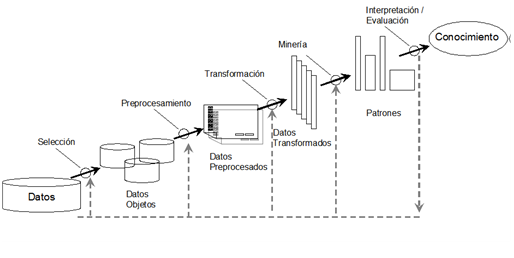
\includegraphics[scale=1]{images/kdd.png}
	\caption[Proceso para el manejo y tratamiento de datos según la metodología KDD.]{Proceso para el manejo y tratamiento de datos según la metodología KDD.\\Fuente: \cite{KDDFigure}}
	\label{fig:procesoKDD}
\end{figure}

\subsection{Herramientas de desarrollo}
\label{subsec:HerrDesarrollo}

A continuación se presentan las herramientas, tanto de \textit{software} como de \textit{hardware} utilizadas para la contrucción del sistema de detección de necesidades.

Se ha se utilizado diversas herramientas de software para la construcción de la aplicación, éstas son descritas a continuación haciendo especial énfasis en aquellas de gran importancia dentro del desarrollo del proyecto

\begin{itemize}
\item Apache Storm: sistema de procesamiento distribuido que basa su procesamiento en dividir el procesamiento en nodos de un grafo dirigido. Permite el procesamiento de eventos en tiempo real.
\item MongoDB: sistema de gestión de bases de datos no-SQL capaz de lidiar con altas tasas de tráfico y respuestas rápidas para aplicaciones en tiempo real.
\item Mallet: biblioteca de Java que contiene herramientas para el procesamiento de lenguaje natural, clasificación de documentos, extracción de información y otras herramientas de aprendizaje automático sobre texto. 
\item Play Framework: \textit{framework} para la contrucción tanto de aplicaciones Java como Scala, utiliza el modelo de arquitectura de diseño modelo-vista-controlador. Está orientado a la construcción de aplicaciones REST y hace hincapié en la productividad de los desarrolladores.
\end{itemize}

Además de las herramientas descritas se hace uso de las una lista de herramientas comunes para el desarrollo de proyectos de \textit{software} presentada a continuación:

\begin{itemize}
\item NetBeans (8.1), como herramienta de apoyo a la construcción de la aplicación.
\item Sublime Text 3 (Build 3103), como editor de textos.
\item MiKTex (XeLaTeX), para la escritura de la memoria.
\item PowerDesigner 16, para la elaboración de diagramas.
\item Bitbucket (Git), como repositorio de todo lo referente al proyecto (detector de necesidades, visualizador y documento de memoria).
\item Windows 10 Home Edition (x64).
\item YourKit 1.8.0\_92 64 bits, para evaluación de \textit{performance} de la aplicación.
\item Linux Mint 17.3 (x86).
\item Oracle VirtualBox (5.0.14).
\end{itemize}

\subsubsection*{Herramientas de \textit{hardware}}
\label{subsubsec:HerrHardw}

Se hace uso del equipo del autor de este trabajo cuyas características técnicas son descritas a contunuación:
\begin{itemize}
\item Procesador Intel Core i5 2.2 Ghz.
\item 8 GB de memoria RAM.
\item 1 TB de disco duro.
\end{itemize}

\section{Organización del documento}
\label{intro:organizacion}

El resto del documento se organiza de la siguiente manera:

El Capítulo \ref{cap:MarcTeorico}, presenta el marco teorico que sustenta la solución implementada y un análisis del estado del arte en términos de las herramientas y tecnicas que han sido utilizadas para dar solucion a problemas similares.

El Capítulo \ref{cap:Requerimientos} describe el proceso de toma de requerimientos de la aplicación. Para ello, siguiendo la metodología XP, se usan de historias de usuario y sus correspondientes criterios de aceptación.

El Capítulo \ref{cap:Diseno}, se presenta la arquitectura del sistema y las decisiones que llevaron a que se se optara por ésta además de describir la implementación de las aplicaciones visualizador y detector de necesidades, incluyendo los elementos que las componen y, en el caso de esta última aplicación, el porqué del uso de una topología en particular.

El Capítulo \ref{cap:experimentos}, describe la completitud de las historias de usuario, evalúa el nivel de replicación de los operadores del sistema y su rendimiento en una simulación de una situación real como fue el terremoto de Concepción en febrero del año 2010.

Finalmente en el Capítulo \ref{cap:conclusiones}, presenta las conclusiones del trabajo realizado, el cumplimiento de objetivos tanto general como específicos, los resultados de los experimentos y trabajo futuro.
\chapter{Marco Teórico}
\label{cap:MarcTeorico}

Este capítulo busca dar a conocer al lector lo último en las áreas que el presente trabajo está inmerso, además de realizar una contextualización de los conceptos necesarios para entender el problema que se está tratando por medio de una breve reseña de cada uno. 

\section{Estado del arte}
\label{intro:motivacion:arte}

Los tópicos que se tratan en esta sección son variados, se comenzará señalando desde donde inicia este trabajo, seguido de las impresiones de distintos autores respecto al trabajo en redes sociales (\textit{Twitter} específicamente), continuando con sistemas de procesamiento para flujos de información para concluir con la construcción de clasificadores para etiquetado de datos.

\subsection{Trabajo previo}
\label{intro:ea:trabajoprevio}

En el marco de las jornadas chilenas de la computación \cite{WladdimiroPMI} propusieron un modelo, desarrollado para el proyecto PMI USA1024, para detectar necesidades de la población ante escenarios de desastres naturales. En se propone un modelo basado en \textit{Yahoo! S4} donde haciendo uso del paradigma de procesamiento de \textit{streams} de datos se forma un grafo cuyos nodos (Elementos de procesamiento o PE, por sus siglas en inglés), dividen el procesamiento en pequeñas tareas fácilmente replicables para paralelizar el \textit{pepeline}. En esa ocación desarrollaron distintos tipos de operadores mencionados a continuación:

\begin{itemize}
\item Recolector: Haciedo uso de la API de \textit{Twitter} obtiene el \textit{stream} de datos del mismo. 
\item \textit{Scheduler}: discrimina cada \textit{tweet} según la categoría que pertenece (Información, agua, electricidad o alimento), mediante el uso de una bolsa de palabras y la distancia \textit{Hamming}.
\item Filtrado: Utiliza un clasificador \textit{Naïve Bayes} para identificar si un \textit{tweet} es subjetivo o no.
\item Relevancia: Identificar si una información es o no confiable haciendo uso de la cantidad de publicaciones del usuario, sus seguidores y a quienes sigue para estimar una reputación del autor.
\item Ranking: Hace uso de la información anterior, decidiendo a qué le entrega mayor importancia.
\end{itemize}

Los autores concluyeron basándose en la carga computacional la importancia de una replicación adecuada para distribuirla entre los PE, pero no fueron concluyentes en cuánto o qué nivel de replicación sería el adecuado o cuándo replicar.

\subsection{La problemática de \textit{Twitter}}
\label{intro:ea:probTwitter}

Diversos autores, entre los que podemos mencionar a \cite{VanDeVoort}, \cite{EventDetectionInTwitter}, \cite{Maldonado}, han señalado las dificultades que se presentan al trabajar utilizando como entradas los estados públicos (\textit{tweet}) de los usuarios de \textit{Twitter}, dentro de las dificultades señaladas se encuentran, por ejemplo, el acceso a la información; si bien existen accesos públicos a la información éstos son restringidos tanto en cantidad como en tiempo: Este punto de acceso permite acceder a un 1\% de la información generada en un instante, es decir, por cada cien \textit{tweets} sólo podra accederse a uno de ellos. Sólo se permite realizar 180 consultas cada quince minutos (aproximadamente 12 consultas por minuto) y, en el caso de ser un usuario identificado, se aumenta a 450 consultas dentro del mismo intervalo de tiempo (aproximadamente 30 consultas por minuto). Por otro lado existe un punto de acceso pagado denominado \textit{FireHose} el cual entrega libre acceso a la información.

Por otro lado \cite{VanDeVoort} señalan que la dificultad radica en el hecho de que cualquier persona puede realizar publicaciones en esta red social, induciendo ruido en la información (considerando el ruido como toda información que aparece junto a la deseada, pero no aporta nueva), además de, al ser publicaciones de máximo 140 caracteres es complejo contextualizar el contenido.

\subsection{Procesamiento de la información}
\label{intro:ea:procesamiento}

Para procesar datos, como los del \textit{stream} de \textit{Twitter}, donde los datos llegan en ráfagas, pueden ser de gran o poco volúmen y requieren de una respuesta inmediata, \cite{HarwoodPeter},hace falta un cambio de paradigma respecto al procesamiento \textit{batch} o procesamiento por lotes, donde un programa ejecuta procesos sin la intervención de terceros desde una base de datos o fichero, por uno donde los datos sean continuos y sin final conocido.
 
Se consideraron tres \textit{frameworks} de computación distribuida: \textit{Apache Storm}, \textit{Apache Spark} y \textit{Apache S4}. El primero presenta una solución basado en el modelo \textit{MapReduce} que toma datos estructurados de la forma (clave, valor) para llevaros a una lista de valores y se usa típicamente para procesar grandes cantidades de datos en distintos nodos que pueden o no estar cercanos físicamente. Los otros dos presentan un modelo basado en el procesamiento de eventos en tiempo real. El problema particular que presenta \textit{S4} es la falta de avances en su desarrollo, el cual ha estado paralizado desde el año 2013. 

\textit{Storm} es un \textit{framework} de computación distribuida para trabajar datos en tiempo real de múltiples fuentes de manera distribuida, tolerante a fallos y de alta disponibilidad. Su funcionamiento se divide en dos elementos: Por un lado existen los \textit{Spout}, encargados de recoger el flujo de entrada de datos, y en segundo, los denominados \textit{bolts}, encajados de procesamiento o transformación de los datos. Por recomendación un \textit{bolt} sólo ha de realizar una tarea. \textit{Storm} puede funcionar de dos formas: En modo \textit{cluster} o modo local; en este último se simula un \textit{thread} por nodo y es utilizado para realizar pruebas locales.

\subsection{Clasificación de textos}
\label{intro:ea:clasificacion}

Por otra parte, la clasificación de texto en servicios de \textit{microblogging}, como \textit{Twitter} es un problema cuya solución tiene diferentes puntos de vista, los métodos tradicionales incluyen hacer uso de una bolsa de palabras para clasificar según el contenido del texto, construcción de n-gramas para clasificar según términos co-ocurrentes o ubicar el texto en una categoría haciendo uso de técnicas de aprendizaje de máquina o \textit{Machine Learning}, \cite{EventDetection}. Éste último método ya ha sido comprobado por diversos autores, entre ellos \cite{Maldonado}, quien utilizó este método para realizar su memoria donde clasificaba \textit{tweets} según sentimientos positivos, negativos o neutros. De igual forma \cite{WladdimiroPMI} utilizaron en su trabajo un clasificador basado en \textit{machine learning} para verificar la subjetividad de un \textit{tweet}, por lo que ya esta demostrado que esta herramienta es capaz de categorizar texto, por lo que puede ser aplicada para las entradas de \textit{Twitter}.

\section{Minería de datos}
\label{sec:dateMine}

A veces llamada como "descubrimiento de información o conocimiento", es el proceso de analizar información de diferentes perspectivas y transformarlo en información de utilidad. Puede ser aplicado a distintas fuentes de datos como: bases de datos, imágenes, internet, etc. Es un campo multidiciplinal que involucra el aprendizaje de máquina, la estadística, bases de datos, la inteligencia artificial y la recuperación de información.

Siendo distintos los usos que pueden dársele se pueden generalizar cuatro etapas:

\begin{itemize}
\item \textbf{Determinación de objetivos}: Delimitar los objetivos que se esperan alcanzar con el proceso de minado.
\item \textbf{Preprocesamiento de datos}: Se refiere a la limpieza, reducción y transformación de las bases de datos. Es, generalmente, el subproceso que utiliza la mayor cantidad de tiempo.
\item \textbf{Determinación del modelo}: Aplicación de algoritmos para generar un modelo que cumpla los objetivos planteados. Se genera nuevo conocimiento o se descubre un patrón.
\item \textbf{Análisis de los resultados}: Se verifica si el conocimiento es útil.
\end{itemize}

Dentro de las tareas que pueden realizarse utilizando \textit{data mining} pueden encontrarse tales como: Aprendizaje supervisado o clasificación, no supervisado o clustering y reglas de asociación.

	\subsection{Minería de la Web}
	\label{subsec:webMine}
	La aplicación de la minería de datos al contenido que se encuentra en línea es conocida como Minería de la \textit{web} o \textit{web mining}. Se diferencia de la minería de datos tradicional en que ésta última utiliza repositorios de datos; en cambio, la minería \textit{web}, hace uso de información extraída directamente desde la \textit{web}.\\
	Sus métodos son similares en cuanto a sus etapas:
	\begin{itemize}
	\item Selección de las fuentes: referencia al proceso de recuperación de los datos.
	\item Selección y pre-procesamiento: Incluye cualquier transformación o pre-procesamiento que puedan realizárseles a los datos, por ejemplo, eliminar elementos, como palabras, aplicación de correctores de datos, etc.
	\item Generalización: Etapa donde se realiza el proceso de minería en sí. 
	\item Análisis: Desarrolla técnicas para utilizar o visualizar el conocimiento adquirido.
	\end{itemize} 

	La información obtenida puede ser utilizara para analizar tanto el contenido de la web (\textit{Web content mining}) como sus enlaces (o relaciones) (\textit{Web  structure mining}) y/o el registro de navegación de los usuarios (\textit{Web usage mining}).

	La primera se refiere a búsqueda entre documentos \textit{web} (texto o imágenes), es decir, analiza los documentos y no la relación entre ellos.

	La segunda se dedica a analizar la topología de los vínculos existentes y/o analizar la estructura interna de la página \textit{web} y descrbir el \textit{HTML} o el \textit{XML} de la misma.

	En particular dentro de la minería de contenido encontramos la minería de texto o \textit{text mining}. Ésta tiene como objetivo el descubrir nueva información a partir colecciones de documentos de texto no estructurado, es decir, texto libre (lenguaje natural, generalmente), aunque también es aceptable otro tipo de información textual como un código fuente. Lo más habitual es trabajar el texto para categorizarlo (Asignar una o más categorías a un documento), clasificarlo (Asignar sólo una clase a un documento) y/o agruparlo (organizar en torno a una jerarquía basado en alguna similitud).

	El primer paso para comenzar a trabajar haciendo uso de minería de texto es representar los datos de alguna manera para luego dárselo a los algoritmos adecuados. Algunas de estas representaciones pueden ser las siguientes:

	\begin{itemize}
	\item Bolsas de palabras (\textit{Bag of words}): Representar el texto como un vector de largo n, donde n corresponde al número de palabras, así cada palabra corresponde a un elemento del vector.
	\item Frases: Considera el texto, simplemente, como una frase sintáctica. Así se permite conservar el contexto.
	\item N-gramas: Consideran la información de la posición de la palabra en el texto mediante secuencias de longitud n (n-gramas). 
	\end{itemize}

	Habiendo realizado la representación, el paso siguiente es reducir el conjunto de características. La literatura indica que los métodos más frecuentados son la eliminación de palabras que no aportan información, llevar las palabras a una palabra raíz (\textit{stemming}), entre otros. \cite{DMPreprocessing}.

\section{Aprendizaje supervisado}
\label{sec:aprendSuperv}

Se caracteriza por ser un proceso de aprendizaje en el que éste se realiza mediante un entrenamiento controlado por un agente externo, el que determina qué respuesta debería generarse a partir de una entrada determinada. \cite{AprendizajeSupervisado}.

Se asocia al concepto de \textit{machine learning} con la minería de datos; la primera busca patrones conocidos y predecir en base a ellos mientras que la segunda busca patrones con anterioridad desconocidos, es decir, la primera tiene una función focalizada en la predicción mientras que la segunda realiza una función exploratoria.

Los datos son denominados instancias, ejemplares, casos o vectores, donde una instancia corresponde a cada uno de los datos disponibles para el análisis.

Los datos poseen atributos son los elementos dentro de las instancias. Una instancia puede tener asociado un elemento de otro conjunto de atributos llamado "Clase", correspondiente a etiquetas de identificación.

Teniendo en cuenta los elementos vistos con anterioridad, se define el objetivo del proceso de aprendizaje como construir una función que relacione las instancias con las clases llamada modelo o, en este caso, clasificador.

Se le llama conjunto de entrenamiento al conjunto de datos utilizado para el aprendizaje. Este conjunto es entregado como entrada al algoritmo de aprendizaje y construcción del modelo. Para realizar la evaluación de la calidad del modelo se utiliza un segundo conjunto de instancias llamado datos de validación. Se espera que estos datos no hayan sido vistos con anterioridad por máquina y así obtener la confianza, es decir, la probabilidad de acierto que calcula el sistema para cada predicción.

Lo ventajoso de este método es que se podrá clasificar una instancia sin haberla visto nunca, pero la desventaja principal es la que han de utilizarse una gran cantidad de instancias para el proceso de entrenamiento. El proceso de entrenamiento y evaluación se ilustra en la Figura ~\ref{fig:entrenamientoEvaluacion}.

\begin{figure}[H]
	\centering
	\captionsetup{justification=centering}
	\includegraphics[scale=0.6]{images/trainTest.png}
	\caption[Proceso de entrenamiento y prueba del modelo.]{Proceso de entrenamiento y prueba del modelo.}
	\label{fig:entrenamientoEvaluacion}
\end{figure}

Dentro de los algoritmos utilizados para la construcción de clasificadores se encuentra \textit{Naïve Bayes} \cite{NaiveBayes2} a continuación se realiza una descripción de este. 

	\subsection{Naïve Bayes}
	\label{subsec:naiveBayes}
	
	La clasificación puede verse como una función \begin{math}\gamma\end{math} que asigna etiquetas a observaciones \cite{NaiveBayes1}, es decir:

	\[\gamma : (x_{1}, .... , x_{n}) \rightarrow \{1, 2, .... r_{0}\} \]

	Existe una matriz de costo \begin{math} cos(r, s)\end{math} con \begin{math} r, s = 1, ...., r_{0}\end{math} en el cual se refleja el costo asociado a las clasificaciones incorrectas. En concreto \begin{math} cos(r, s) \end{math} indica el costo de clasificar un ejemplo de la clase r como de la clase s. En el caso especial de la función de pérdida 0/1, se tiene:

	\[ cos(r, s) = \left \{ \begin{matrix} 0 & \mbox{si }r \ne s
\\ 1 & \mbox{si }r = s \end{matrix}\right. \]

	Subyacente a las observaciones suponemos la existencia de una distribución de probabilidad conjunta:

	\[
		p(x_{1}, ..., x_{n}, c) = p(c | x_{1}, ..., x_{n})p(x_{1}, ..., x_{n}) = p(x_{1}, ..., x_{n}|c)p(c)
	\]

	La cual es desconocida. El objetivo es construir un clasificador que miniza el coste total de los errores cometidos, y esto se consigue, \cite{NaiveBayes3} por medio del clasificador de Bayes:

	\[
		\gamma(x) = arg min_{\substack{k}} \sum^{r_{0}}_{\substack{c = 1}} cos(k,c)p(c | x_{1}, ..., x_{n})
	\]

	En el caso que la función de pérdida sea 0/1, el clasificador de Bayes se convierte en asignar al ejemplo \begin{math} x = (x_{1}, ..., x_{n})\end{math} la clase con mayor probabilidad a posteriori. Es decir:

	\[
		\gamma(x) = arg max_{\substack{c}} p(c | x_{1}, ..., x_{n})
	\]

	En la práctica la función de distribución conjunta \begin{math} p(x_{1}, ..., x_{n}, c) \end{math} es desconocida, y puede ser estimada a partir de una muestra aleatorea simple \begin{math} \{ (x^{(1)}, c^{(1)} ), ..., (x^{(N)}, C^{(N)})\}\end{math} extraida de dicha función de distribución conjunta.

	El paradigma clasificatorio en el que se utiliza el teorema de Bayes en conjunción con la hipótesis de independencia condicional de las variables predictorias dada la clase se conoce como Naïve Bayes, \cite{NaiveBayes3}.

	Finalmente el Teorema de Bayes está representado por la expresión \cite{NaiveBayes4}:

	\[
		P(c_{i}|d_{j}) = \frac{P(d_{j}|c_{i}) · P(c_{i})}{P(d_{j})}
	\]

	Donde \begin{math} c_{i} \end{math} corresponde al atributo Clase y \begin{math} d_{j} \end{math} al conjunto de documentos. El término \begin{math} P(d_{j}) \end{math} suele omitirse, pues no aporta mucha información para la clasificación. Habiendo realizado lo anterior y tomando en cuenta la hipótesis de independencia se obtiene:

	\[
		P(d_{j}|c_{i}) = P(c_{i})\prod_{j=1}^n P(a_{j}|c_{i})
	\]

	Pero siempre se considera la mayor probabilidad de \begin{math} c_{i} \end{math}, por ello podemos añadir un nuevo elemento llegando a la fórmula de Naïve Bayes:

	\[
		P(d_{j}|c_{i}) = ArgMax{\substack{k}^n P(c_{i})}\prod_{j=1}^n P(a_{j}|c_{i})
	\]

	En términos simples el crear un modelo de clasificación Naïve Bayes se puede resumir en el Algoritmo \ref{alg:NaiveB}.

	\begin{algorithm}[H]\setstretch{1.5}
	\begin{algorithmic}[numeracion_lineas]
		\REQUIRE Clases $C=\{c_{0}, \dots, c_{n} \}$.
		\REQUIRE Datos de entrenamiento $D= \{d_{0}, \dots, d_{n} \}$
		\ENSURE Modelo de clasificación $M$.

		\FOR{Clase $c_{i}$ perteneciente a $C$}
			\STATE Calcular las probabilidades a priori para cada clase (Probabilidad de que un dato cualquiera pertenezca a $c_{i}$.
		\ENDFOR

		\FOR{Clase $c_{i}$ perteneciente a $C$}
			\STATE Realizar un recuento de los valores $v_{i}$ de atributos que toma cada ejemplo $d_{i}$, guardarlos en $V$.
		\ENDFOR

		\FOR{Valores $v_{i}$ perteneciente a $V$}
			\STATE Aplicar corrección de Laplace a $v_{i}$.
		\ENDFOR

		\FOR{Valores $v_{i}$ perteneciente a $V$}
			\STATE Normalizar para obtener un rango de valores [0,1].
		\ENDFOR

	\end{algorithmic}
	\caption{Algoritmos Naïve Bayes.}
	\label{alg:NaiveB}
	\end{algorithm}\vphantom\\

	Para utilizar el modelo generado por el Algoritmo \ref{alg:NaiveB}, se hace uso del Algoritmo \ref{alg:NaiveBAplic} sobre un dato de entrada $d_{j}$.

	\begin{algorithm}[H]\setstretch{1.5}
	\begin{algorithmic}[numeracion_lineas]
		\REQUIRE Clases $C=\{c_{0}, \dots, c_{n} \}$.
		\REQUIRE Dato $d_{j}$.
		\ENSURE Etiqueta del Dato $d_{i}$.

		\FOR{Clase $c_{i}$ perteneciente a $C$}
			\STATE Calcular las probabilidades a priori para cada clase (Probabilidad de que un dato cualquiera pertenezca a $c_{i}$.
		\ENDFOR

		\STATE retornar $ArgMax{\substack{k}^n P(c_{i})}\prod_{j=1}^n P(d_{j}|c_{i})$.

	\end{algorithmic}
	\caption{Algoritmos Naïve Bayes.}
	\label{alg:NaiveBAplic}
	\end{algorithm}\vphantom\\
	

\section{Metodología}
\label{sec:MetodologiaDetalle}

Para la realización de este trabajo se utilizarán dos metodologías, en esta sección se ambas son definidas.

\subsection{Programación Extrema}
\label{subsec:XP}

La Programación Extrema (\textit{Extreme Programming}, XP desde ahora en adelante), comenzó como un proyecto el 6 de Marzo de 1996. Es uno de los procesos ágiles más populares y ha sido provado exitosamente en compañias e industrias de todos los tamaños. \cite{xP}.

Su éxito se debe a que hace especial incapié en la satisfacción del cliente por sobre la entrega de todo lo el software posible.

Aporta cinco formas escenciales para mejorar el proceso de desarrollo de software: Comunicación, simplicidad, retroalimentación, respeto y coraje: Constantemente se comunica al equipo de desarrollo con el cliente. Se intenta mantener el diseño lo más simple y sencillo posible. Se obtiene retroalimentación desde las pruebas desde el día uno. Se les entrega el software al cliente lo más pronto posible con los cambios solicitados. El éxito depende, en gran medida, del respeto y comunicación de los miembros del equipo y los clientes. Implementando XP el equipo puede responder a los cambios sin temor.

La metodología implementa unas simples reglas de trabajo, las que se dividen en cinco grandes áreas las que se detallarán a continuación.

\begin{enumerate}
\item Planeación:
	\begin{itemize}
	\item Se escriben Historias de usuario. 
	\item Se crea un plan de \textit{releases}.
	\item Se planifican liberaciones pequeñas y frecuentes.
	\item Se divide el proyecto en iteraciones.
	\item Al comienzo de cada iteración se planea cómo será.
	\end{itemize}
\item Manejo:
	\begin{itemize}
	\item Se le da al equipo una área de trabajo.
	\item Se realizan reunione del tipo \textit{stand up meeting} a díario.
	\item Se mide la velocidad del proyecto. 
	\item Se mueven a las personas de sus puestos (para que todo el equipo pueda trabajar en todo).
	\item Se solucionan problemas que instroduzcan quiebres en la metodología.
	\end{itemize}
\item Diseño:
	\begin{itemize}
	\item Simplicidad. El mejor diseño es el más simple.
	\item Se crean \textit{spikes} para reducir el riesgo.
	\item No se agregan funcionalidades antes de tiempo.
	\item Hacer uso de técnicas de \textit{refactoring}, cada vez que sea posible.
	\end{itemize}
\item Implementación:
	\begin{itemize}
	\item El cliente siempre está disponible. 
	\item El código debe ser escrito bajo estándares. 
	\item Se hace uso de \textit{Test Driven Development }(TDD).
	\item Todo el código debe hacerse haciendo uso de \textit{pair programming}.
	\item Sólo una pareja integra código a la vez.
	\item Integración a menudo.
	\item Se cuenta con un equipo dedicado a la integración.
	\item El código es de todos.
	\end{itemize}
\item Prueba:
	\begin{itemize}
	\item Todo el código debe tener pruebas unitarias.
	\item Todas las pruebas deben ser pasadas antes de una liberación.
	\item Cuando se encuentra un \textit{bug}, se crean pruebas.
	\item Los \textit{test} de aceptación se corren a menudo y sus resultados son publicados.
	\end{itemize}
\end{enumerate}

Éstas reglas por si solas pueden carecer de sentido, pero se apoyan en los \textbf{valores} que la metodología quiere entregar y que fueron mencionadas anteriormente, pero ahora son detalladas:

\begin{itemize}
\item Simplicidad: Se hará lo que se solicitó, pero no más. Ésto maximiza el valor entregado dado una fecha límite. Nuestras metas se alcanzarán por medio de pequeños pasos para mitigar errores tan pronto ocurran. Crearemos algo de lo que estemos orgullosos y lo mantendremos en el tiempo a costos razonables.
\item Comunicación: Todos somos partes de un equipo y nos comunicamos cara a cara a diario. Trabajaremos juntos en todo: desde la toma de requerimientos hasta la implementación. Crearemos la mejor solución posible al problema.
\item Retroalimentación: Cada iteración será completada seriamente entregando \textit{software} funcional. Mostraremos nuestro \textit{software} a menudo y prontamente para luego escuchar y aplicar los cambios solicitados. Hablaremos de nuestro proyecto y adaptaremos nuestro proceso a el, no al revéz.
\item Respeto: Todos dan y reciben el respeto que merecen como miembros del equipo. Todos contribuyen con valor así sea simple entusiasmo. Los desarrolladores respetan la experiencia del cliente y viceversa. 
\item Coraje: Diremos la verdad sobre el progreso y nuestras estimaciones. No se documentan excusas por si se falla porque se planea tener éxito. No tenemos porque no trabajamos solos. Nos adaptaremos a los cambio cuando ocurran.
\end{itemize}

El proceso de XP puede puede ser aprecido en la Figura \ref{fig:procesoXP}.

\begin{figure}[H]
	\centering
	\captionsetup{justification=centering}
	\includegraphics[scale=0.6]{images/flowChartXP.png}
	\caption[Diagrama de flujo de Programación Extrema.]{Diagrama de flujo de Programación Extrema}
	\label{fig:procesoXP}
\end{figure}

\subsection{\textit{Knowledge Discovery in Databases} (KDD)}
\label{subsec:kdd}

Es definido por \cite{KDDFayyad} como "El proceso no trivial de identificar patrones válidos, nuevos, potencialmente útiles y en ultima instancia comprensible en los datos", surge de la necesidad de manejar grandes cantidades de datos e involucra simultaneamente varias disciplinas de investigación tales como el aprendizaje automático, la estadística, inteligencia artificial, sistemas de gestión de bases de datos, sistemas de apoyo a la toma de decisiones, entre otras.

Si bien puede variar el usuario, quien es aquel que determina el domino de la aplicación, es decir, cómo se utilizarán los datos, el proceso generalmente considera las siguientes etapas:

\begin{enumerate}
\item Selección de datos: Consiste en buscar el objetivo y las herramientas del proceso de minería, identificando los datos que han de ser extraídos, buscando atributos apropiados de entrada y la información de salida para representar la tarea. Esto quiere decir, primero se debe tener en cuenta lo que se sabe, lo que se quiere obtener y cuáles son los datos que nos facilitarán esa información para poder llegar a nuestra meta, antes de comenzar el proceso como tal.
\item Limpieza de datos: En este paso se limpian los atributos sucios, incluyendo datos incompletos, el ruido y datos inconsistentes. Estos datos sucios, en algunos casos, deben ser eliminados, pues pueden contribuir a un análisis inexacto y resultados incorrectos.
\item Integración de datos: Combina datos de múltiples procedencias incluyendo múltiples bases de datos, que podrían tener diferentes contenidos y formatos.
\item Transformación de datos: Consiste en modificaciones sintácticas llevadas a cabo sobre los datos sin que suponga un cambio en la técnica de minería aplicada. Tiene dos caras, por un lado existen ventajas en el sentido de mejorar la interpretación de las reglas descubiertas y reduce el tiempo de ejecución, por el otro puede llevar a la pérdida de información.
\item Reducción de datos: Reducción del tamaño de los datos, encontrando características más significativas dependiendo del objetivo del proceso.
\item Minería de datos: Consiste en la búsqueda de patrones de interés que puedan expresarse como un modelo o dependencia de los datos. Se ha de de especificar un criterio de preferencia para seleccionar un modelo de un conjunto de posibles modelos. Además se ha de especificar la estrategia de búsqueda (algoritmo), a utilizar.
\item Evaluación de los patrones: Se identifican patrones interesantes que representan conocimiento utilizando diferentes técnicas incluyendo análisis estadísticos y lenguajes de consulta.
\item Interpretación de resultados: Consiste en entender resultados de análisis y sus implicaciones y puede llevar a regresar a algunos pasos anteriores.
\end{enumerate}

La representacíón del proceso descrito por la metodología KDD puede verse esquematizado en la Figura \ref{fig:procesoKDD}.

\begin{figure}[H]
	\centering
	\captionsetup{justification=centering}
	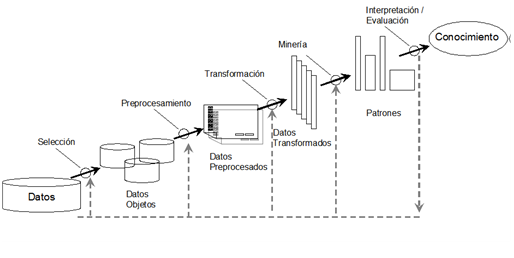
\includegraphics[scale=1]{images/kdd.png}
	\caption[Proceso KDD.]{Proceso KDD.}
	\label{fig:procesoKDD}
\end{figure}

\section{Herramientas}
\label{sec:herramientas}

	Esta sección busca dar a conocer al lector las herramientas de \textit{software} utilizadas para desarrollar el sistema propuesto.

	\subsection{Play Framework}
	\label{subsec:playframework}

	Es un \textit{framework} de código abierto para aplicaciones \textit{web} escrito en \textit{Java} y \textit{Scala}, el cual sigue el patrón de arquitectura \textit{Modelo-Vista-Controlador} (MVC). Utiliza el paradigma de diseño "Convención sobre configuración", el cual apunta a reducir la toma de decisiones que debe tomar el desarrollador sin perder flexibilidad. 

	Se enfoca en la productividad a aplicaciones \textit{RESTful}.

	Elimina la desventaja de desarrollo al utilizar \textit{Java} dada por el continuo ciclo de compilar-empaquetamiento-despliegue. Al detectar cambios en el código realiza inmediatamente la compilación y actualiza en la JVM sin necesidad de reiniciar el servidor.

	Play no utilizar sesiones en su funcionar, privilegiando el uso de almacenamiento \textit{offline} o el uso de peticiones \textit{Ajax} para resolver problemas del lado del cliente.

	\subsection{Apache Storm}
	\label{subsec:apacheStorm}

	Apache Storm es un sistema de computación en tiempo real de código abierto. Simplifica el problema de flujos (\textit{streams}), de datos sin que estos tengan fin.

	Es escalable, tolerante a fallos y garantiza que toda la información será procesada. Presenta \textit{Benchmarks} que señalan que por nodo es capaz de procesar más de un millón de tuplas por segundo.

	Se compone principalmente de dos partes. La primera es denominada \textit{Spout} y es la encargada de recoger el flujo de datos de entrada. La segunda es denominada \textit{Bolt} y es la encargada de la transformación o procesado de los datos.

	Oficialmente es representado como puede verse en la Figura \ref{fig:stormBeLike}. donde los \textit{Spouts} son representados simulando ser llaves de agua desde donde fluyen los datos al sistema y los \textit{Bolts} como rayos donde se procesa el flujo.

	\begin{figure}[H]
		\centering
		\captionsetup{justification=centering}
		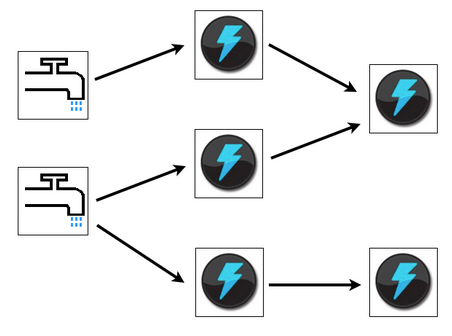
\includegraphics[scale=0.6]{images/stormBeLike.png}
		\caption[Representación del funcionamiento de Apache Storm.]{Representación del funcionamiento de Apache Storm.}
		\label{fig:stormBeLike}
	\end{figure}

	Uno de los puntos fuertes que tiene este sistema es que al crear una topología donde se instancian \textit{Bolts} y \textit{Spouts}, Storm se encarga de escalar el sistema distribuyendo los elementos en sus componentes.

	Al trabajar con \textit{Apache Storm}, como ya se ha descrito, se han de construir dos elementos: \textit{spout} y \textit{bolt}. Éstos elementos se construyen realizando heredando desde desde \textit{BaseRichSpout}, para el caso de \textit{spout} e implementando \textit{IRichBolt} para los \textit{bolt}. La descripción de los elementos de éstas clases se presentan en las secciones \ref{subsubsec:Spout} y \ref{subsubsec:Bolt}.

	\subsubsection{Spout}
	\label{subsubsec:Spout}

	\begin{figure}[H]
		\centering
		\captionsetup{justification=centering}
		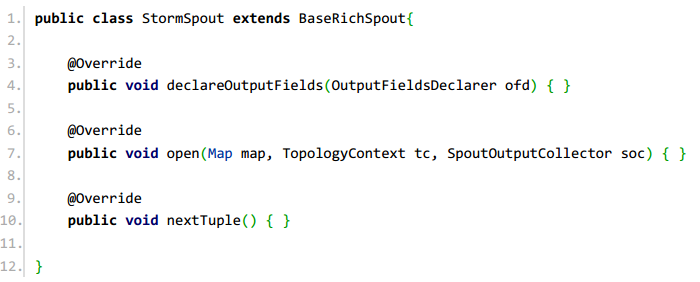
\includegraphics[scale=0.8]{images/SpoutBase.png}
		\caption[Construcción de un Spout.]{Construcción de un Spout.}
		\label{fig:spoutbase}
	\end{figure}

	En la figura \ref{fig:spoutbase} muestra la base para la implementación de un \textit{spout}. Cuenta con tres métodos:

	\begin{itemize}
	\item \textit{declareOutputFields}: declara nombres para las etiquetas que tendrá el objeto emitido.
	\item \textit{open}: Inicializa todos los elementos utilizados en el spout.
	\item \textit{nextTuple}: es llamado desde storm al recibir una nueva tupla para realizar una tarea.
	\end{itemize}	

	\subsubsection{Bolt}
	\label{subsubsec:Bolt}

	\begin{figure}[H]
		\centering
		\captionsetup{justification=centering}
		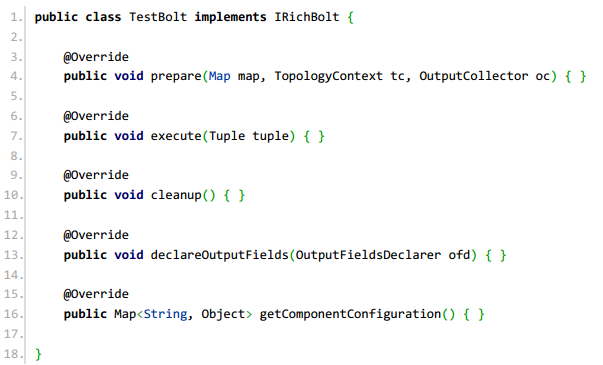
\includegraphics[scale=0.8]{images/BoltBase.png}
		\caption[Construcción de un Bolt.]{Construcción de un Bolt.}
		\label{fig:boltbase}
	\end{figure}

	La figura \ref{fig:boltbase} presenta la base para la implementación de un \textit{bolt}. Sus métodos se explican a continuación:

	\begin{itemize}
	\item \textit{prepare}: Similar al método \textit{open} para los \textit{spout}, realiza la misma función.
	\item \textit{execute}: Cumple la misma función que el método \textit{nextTuple}.
	\item \textit{cleanup}: Al finalizar una topología se llama este método para cerrar el \textit{bolt}.
	\item \textit{declareOutputFields}: declara nombres para las etiquetas que tendrá el objeto emitido.
	\item \textit{getComponentConfiguration}: Usado al querer cambiar una configuración del sistema.
	\end{itemize}

	\subsubsection{Topología}
	\label{subsubsec:topologia}

	Una topología de Storm es similar a un grafo. Cada nodo se encarga de procesar una determinada información y le pasa el testigo al siguiente nodo. Está compuesta por \textit{Spouts} y \textit{Bolts}. \cite{Storm}.

	\subsubsection{Cluster de Storm}
	\label{subsubsec:clusterStorm}

	Un cluster de Storm no muere, se queda siempre en espera de nuevos datos de entrada mientras el proceso siga activo.

	La arquitectura de Storm se divide en tres componentes:
	\begin{itemize}
	\item Master Node: Ejecuta el demonio llamado Nimbus, el cual es responsable de distribuir el código a través del cluster. Realiza la asignación y monitorización de tareas en las distintas máquinas del cluster.
	\item Worker Node: Ejecutan el demonio Supervisor, el cual se encarga de recoger y procesar los trabajos asignados en la máquina donde está corriendo. En caso de fallo de uno \textit{Worker Node}, Nimbus se dará cuenta y redirigirá el trabajo a otro.
	\item Zookeeper: Si bien no es un componente propio de Storm, es necesario para su funcionamiento, pues se encarga de coordinar Nimbus y Supervisor, además de mantener sus estados, pues ambos son \textit{stateless}.
	\end{itemize}

	\subsubsection{Modos de funcionamiento}
	\label{subsubsec:modoFuncionamientoStorm}

	Storm puede funcionar de dos modos: Local y Cluster. El primero es útil para el desarrollo, pues ejecuta toda la topología en una única JVM, por lo que pueden realizarse fácilmente pruebas de integración, depurar código, etcétera. Este modo simula, haciendo uso de \textit{Threads}, cada nodo del Cluster. \cite{Storm}.

	El modo Cluster es considerado el 'modo de producción' y es el modo donde el código es distribuido en máquinas diferentes dentro del Cluster.

	\subsubsection{Storm grouping}
	\label{subsubsec:StormGrouping}

	Se refiere a la forma en la que se van a compartir los datos entre los componentes. Como modelo de datos, Storm utiliza tuplas que son listas de valores con un nombre específico. El valor puede ser cualquier tipo, para ello se ha de implementar un serializador. \cite{Storm}.

	\begin{itemize}
	\item Shuffle grouping: Storm decide de forma \textit{round robin} la tarea a la que se va a enviar la tupla, de manera que la distribución sea equivalente entre todos los nodos.
	\item Fields gruoping: Se agrupan los \textit{streams} por un determinado campo de manera que se distribuyen los valores que cumplen una determinada condición a la misma tarea.
	\item All grouping: El \textit{stream} pasa por todas las tareas haciendo multicast.
	\item Grobal grouping: El \textit{stream} se envía al \textit{bolt} con ID más bajo.
	\item None grouping: Es un \textit{Shuffle grouping} donde el orden no es importante.
	\item Direct grouping: La tarea es la encargada de decidir hacia donde emitir especificando el ID del destinatario.
	\item Local grouping: Se utiliza el mismo \textit{bolt} si tiene una o más tareas en el mismo proceso.
	\end{itemize}

	\subsection{MongoDB}

	Base de datos no relacional (NoSQL) de código abierto escrita en C++ y está orientada al trabajo en documentos. Lo anterior quiere decir que, en lugar de guardar los datos en registros, lo hace en documentos y éstos son almacenada en una representación binaria de JSON conocida como BSON.

	Una de las diferencias fundamentales con respecto a las bases de datos relacionales es que no es necesario que se siga un esquema; en una misma colección - concepto similar a una tabla en las bases de datos relacionales - pueden tener distintos esquemas.

	MongoDB fue creado para brindar escalabilidad, rendimiento y disponibilidad. Puede ser utilizado en un servidor único como en múltiples. Esto se logra dado que MongoDB brinda un elevado rendimiento, tanto para lectura como para escritura, potenciando la computación en memoria.

	Las consultas en MongoDB se realizan como si se tratase de Javascript entregando como parámetro un objeto JSON. Por ejemplo, dado el documento presentado en la Figura ~\ref{fig:MongoJsonExample}, parte de una colección llamada 'Personas' en MongoDB:

	\begin{figure}[H]
		\centering
		\captionsetup{justification=centering}
		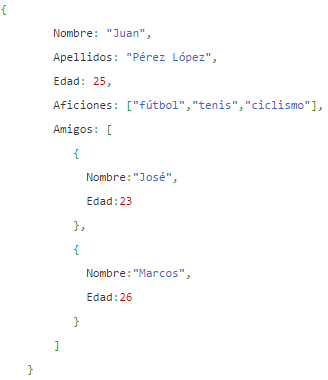
\includegraphics[scale=0.8]{images/MongoJsonExample.png}
		\caption[Documento en MongoDB.]{Documento en MongoDB.}
		\label{fig:MongoJsonExample}
	\end{figure}

	Una consulta para encontrar este elemento dentro de la colección se daría de la forma aprecida en la Figura ~\ref{fig:MongoJsonQueryExample}

	\begin{figure}[H]
		\centering
		\captionsetup{justification=centering}
		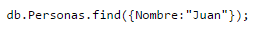
\includegraphics[scale=0.8]{images/MongoJsonQueryExample.png}
		\caption[Consulta en MongoDB.]{Consulta en MongoDB.}
		\label{fig:MongoJsonQueryExample}
	\end{figure}

	En pruebas realizando operaciones habituales dentro de las bases de datos \cite{MongoPerformance} demostró que el tiempo de ejecución de MongoDB, como base de datos NoSQL, aventaja significativamente a las bases de datos relacionales más populares como lo son MySQL y PostgreSQL.


	
\chapter{Requerimientos}
\label{cap:Requerimientos}

Éste capítulo detalla los requisitos de las aplicaciones, descritos como historias de usuario. Éstos señalan las necesidades de los clientes.

El cliente es uno de los clientes del proyecto FONDEF IDeA, código ID15I10560, proyecto orientado a generar herramientas para la gestión de desastres naturales. Los requerimientos se levantan en reuniones con los investigadores y responsables de aplicaciones del proyecto donde se estipulan las funcionalidades deseables, dichas reuniones tuvieron lugar en el Departamente de Ingeniería informática de la Universidad de Santiago e Chile.

\section{Proceso de toma de requerimientos}
\label{sec:tomaDeRequerimientos}

Las primeras reuniones tuvieron un caracter exploratorio, en ellas se discutieron aspectos referentes al estado del arte y se acotaron los alcances del proyecto. En reuniones subsecuentes y mediante conversaciones con el equipo del proyecto FONDEF IDeA se encontraron los requisitos descritos en la tabla \ref{tab:requerimientos} mediante los cuales fue posible construir las historias de usuarios necesarias para la metodología que se está empleando. Los requisitos mostrados a continuación se corresponden con el identificador RFXX para los requerimientos funcionales, donde XX corresponde al número del requisitos y RNFYY, para el caso de los requerimientos no funcionales donde YY corresponde al número del requisito.

\begin{table}[]
\centering
\caption[Requisitos encontrados]{Requisitos encontrados\\Fuente: Elaboración Propia, (2016)}
\label{tab:requerimientos}
\begin{tabular}{|c|l|c|}
\hline
\textbf{Identificador} & \multicolumn{1}{c|}{\textbf{Requisito}} & \textbf{Dependencia} \\ \hline
RNF00 & \begin{tabular}[c]{@{}l@{}}Se ha de implementar un sistema de procesamiento\\ de \textit\{streams\}.\end{tabular} & - \\ \hline
RNF01 & La fuente de datos debe ser \textit\{Twitter\}. & - \\ \hline
RNF02 & \begin{tabular}[c]{@{}l@{}}Debe obtenerse la información de \textit\{Twitter\}\\ en tiempo real.\end{tabular} & RNF01 \\ \hline
RNF03 & El sistema debe ser escalable & RNF00 \\ \hline
RNF04 & \begin{tabular}[c]{@{}l@{}}El sistema debe presentar una interfaz donde el\\ usuario pueda opearar.\end{tabular} & - \\ \hline
RNF05 & \begin{tabular}[c]{@{}l@{}}La interfaz debe poder recargar su información \\ sin actualizar la misma\end{tabular} & RNF04 \\ \hline
RNF06 & \begin{tabular}[c]{@{}l@{}}Los parámetros utilizados para operar el sistema \\ deben ser modificables.\end{tabular} & - \\ \hline
RNF07 & \begin{tabular}[c]{@{}l@{}}Se debe presentar un mapa para el despliegue de\\ la información.\end{tabular} & RNF04 \\ \hline
RNF08 & Cada categoría debe tener un icono particular. & RF05 \\ \hline
RNF09 & \begin{tabular}[c]{@{}l@{}}La información en el mapa debe agruparse según\\ nivel de acercamiento de éste.\end{tabular} & RNF08, RNF04 \\ \hline
RNF10 & \begin{tabular}[c]{@{}l@{}}Se debe poder elegir qué eventos se muestran por\\ categoría\end{tabular} & RNF08, RNF04 \\ \hline
RNF11 & \begin{tabular}[c]{@{}l@{}}Se deben mostrar estadísticas de procesamiento \\ para la consulta actual.\end{tabular} & RF02, RNF04 \\ \hline
RNF12 & \begin{tabular}[c]{@{}l@{}}Se debe mostrar desde donde viene un evento, es \\ decir, qué estado lo generó al visualizarlo en el\\ mapa.\end{tabular} & \begin{tabular}[c]{@{}c@{}}RNF10, RNF09,\\ RNF04\end{tabular} \\ \hline
RNF13 & \begin{tabular}[c]{@{}l@{}}Debe mostrarse una línea temporal para seleccionar\\ el intervalo.\end{tabular} & RF08 \\ \hline
RNF14 & \begin{tabular}[c]{@{}l@{}}Debe mostrarse un histograma con la cantidad de\\ eventos pasado por fecha.\end{tabular} & RF08 \\ \hline
RF00 & \begin{tabular}[c]{@{}l@{}}Se deben detectar las necesidades expresadas\\ en los \textit\{tweets\}\end{tabular} & \begin{tabular}[c]{@{}c@{}}RNF00, RNF01,\\ RNF02\end{tabular} \\ \hline
RF01 & \begin{tabular}[c]{@{}l@{}}Los operadores del sistema deben especificarse\\ como \textit\{bolts\}\end{tabular} & RNF00 \\ \hline
RF02 & Se debe poder especificar términos de búsqueda, & RNF00, RNF04, \\ \hline
RF03 & \begin{tabular}[c]{@{}l@{}}Los términos ingresados deben expandirse,\\ automáticamente, para abarcar nuesvos términos\\ útiles.\end{tabular} & RF03 \\ \hline
RF04 & Sólo se trabajaran \textit\{tweets\} en español. & RF01, RNF00 \\ \hline
RF05 & \begin{tabular}[c]{@{}l@{}}La detección de necesidades debe realizarse de \\ forma dinámica, no utilizando bolsas de palabras.\end{tabular} & - \\ \hline
RF06 & Se debe poder acceder a eventos pasados. & - \\ \hline
RF07 & Debe existir un sistema de persistencia de datos. & RF06 \\ \hline
RF08 & \begin{tabular}[c]{@{}l@{}}Se debe poder especificar un intervalo dentro del \\ cual mostrar datos.\end{tabular} & RF06 \\ \hline
RF09 & El sistema debe funcionar de forma continua & - \\ \hline
\end{tabular}
\end{table}

\section{Historias de usuario y criterios de aceptación}
\label{sec:historias}

Los requerimientos antes mencionados se agruparon para, según lo descrito por la metodología \textit{extreme programming}, como historias de usuario. Estas historias de usuario tienen la siguiente nomenclatura para su identificación: Aquellos que guarden relación con la aplicación de detección se identifican como 'HU-cXX', donde XX corresponde al número del requisito; 'HU-vYY' para aquellas que correspondan a la aplicación interfaz, donde, al igual que en el caso anterior, YY corresponden al número del requisito.

La Tabla \ref{tab:ReqTotales} presenta las historias de usuario correspondientes a los requerimientos de todo el sistema en general, sin hacer referencia al cómo está dividido éste.

\begin{table}[H]
\centering
\caption[Historias de usuario.]{Historias de usuario.\\Fuente: Elaboración Propia, (2016)}
\label{tab:ReqTotales}
\begin{tabular}{cl}
\hline
\textbf{Identificador}       & \multicolumn{1}{c}{\textbf{Historia de usuario}}                                                                                                                                                                                                                                                                                                                                      \\ \hline
\multicolumn{1}{|c|}{HU-c00} & \multicolumn{1}{l|}{\begin{tabular}[c]{@{}l@{}}Como cliente quiero capturar necesidades de la población en tiempo real \\ cuando el país se encuentre en un escenario de catástrofe natural para poder \\ contar con información para asistir a la población afectada.\end{tabular}}                                                                                                  \\ \hline
\multicolumn{1}{|c|}{HU-c01} & \multicolumn{1}{l|}{\begin{tabular}[c]{@{}l@{}}Como cliente quiero que las necesidades detectadas se recojan desde la \\ información generadas en redes sociales redes sociales para que las personas\\ sean la fuente primaria.\end{tabular}}                                                                                                                                        \\ \hline
\multicolumn{1}{|c|}{HU-c02} & \multicolumn{1}{l|}{\begin{tabular}[c]{@{}l@{}}Como cliente quiero que la búsqueda de necesidades se vea enriquecida para\\  abarcar nuevos términos de búsqueda para abarcar un conjunto mayor de \\ información.\end{tabular}}                                                                                                                                                      \\ \hline
\multicolumn{1}{|c|}{HU-v00} & \multicolumn{1}{l|}{\begin{tabular}[c]{@{}l@{}}Como usuario quiero una interfaz donde pueda visualizar el comportamiento \\ del sistema de detección para poder interactuar con el.\end{tabular}}                                                                                                                                                                                     \\ \hline
\multicolumn{1}{|c|}{HU-v01} & \multicolumn{1}{l|}{\begin{tabular}[c]{@{}l@{}}Como cliente quiero que las necesidades detectadas puedan ser asociadas a \\ un punto en un mapa geográfico para poder identificar el lugar físico de su \\ fuente.\end{tabular}}                                                                                                                                                      \\ \hline
\multicolumn{1}{|c|}{HU-v02} & \multicolumn{1}{l|}{\begin{tabular}[c]{@{}l@{}}Como usuario quiero que puedan aplicarse filtros a la visualización de los \\ puntos de modo que según la distancia entre ellos, cuáles se quieran mostrar\\ y el nivel de acercamiento que tenga el mapa se entreguen diferentes formas\\ de mostrar la información para que la información se visualice con facilidad.\end{tabular}} \\ \hline
\multicolumn{1}{|c|}{HU-v03} & \multicolumn{1}{l|}{\begin{tabular}[c]{@{}l@{}}Como usuario quiero que la visualización de eventos se realice en tiempo \\ real para tomar decisiones rápidas cuando la situación lo amerite.\end{tabular}}                                                                                                                                                                           \\ \hline
\multicolumn{1}{|c|}{HU-v04} & \multicolumn{1}{l|}{\begin{tabular}[c]{@{}l@{}}Como usuario quiero visualizar eventos pasados, además quiero poder \\ seleccionar un intervalo de tiempo y que el sistema muestre todos los \\ eventos que se hayan detectado dentro de aquel intervalo de modo que \\ pueda realizarse una análisis a posteriori de la emergencia.\end{tabular}}                                     \\ \hline
\multicolumn{1}{|c|}{HU-v05} & \multicolumn{1}{l|}{\begin{tabular}[c]{@{}l@{}}Como usuario quiero poder especificar términos de búsqueda para acotar la\\  búsqueda a aquel contenido que contenga elementos que se correspondan \\ con ellos.\end{tabular}}                                                                                                                                                         \\ \hline
\multicolumn{1}{|c|}{HU-v06} & \multicolumn{1}{l|}{\begin{tabular}[c]{@{}l@{}}Como usuario quiero que cada punto, correspondiente a una necesidad \\ específica, tenga un diseño particular fácilmente identificable.\end{tabular}}                                                                                                                                                                                  \\ \hline
\multicolumn{1}{|c|}{HU-07}  & \multicolumn{1}{l|}{\begin{tabular}[c]{@{}l@{}}Como usuario quiero que sea posible visualizar estadísticas del procesamiento\\ de la aplicación por consulta.\end{tabular}}                                                                                                                                                                                                           \\ \hline
\multicolumn{1}{|c|}{HU-08}  & \multicolumn{1}{l|}{\begin{tabular}[c]{@{}l@{}}Como usuario quiero poder modificar cuánto tiempo se visualizará un evento \\ antes de que sea considerado antiguo y cada cuánto tiempo se ha de añadir la\\ información de los nuevos eventos.\end{tabular}}                                                                                                                               \\ \hline
\end{tabular}
\end{table}

Estas historias de usuario se corresponden con los criterios de aceptación descritos en la Tabla \ref{tab:criteriosAceptacion} que se presenta a continuación.

\begin{table}[H]
\centering
\caption[Criterios de aceptación.]{Criterios de aceptación.\\Fuente: Elaboración Propia, (2016)}
\label{tab:criteriosAceptacion}
\begin{tabular}{|c|l|}
\hline
\textbf{Identificador} & \multicolumn{1}{c|}{\textbf{Criterio de aceptación}} \\ \hline
HU-c00 & \begin{tabular}[c]{@{}l@{}}· Debe contruirse el sistema de procesamiento de stream.\\ · Debe capturarse la información desde Twitter.\\ · Debe usarse la información que llega al sistema y no almacenarla para\\ trabajarla por lotes.\\ · El sistema debe concluir con un dato etiquetado en la base de datos.\end{tabular} \\ \hline
HU-c01 & · Twitter debe ser desde donde se obtienen los datos de entrada del sistema. \\ \hline
HU-c02 & · Deben implementarse técnicas para realizar expansión de la consulta. \\ \hline
HU-v00 & \begin{tabular}[c]{@{}l@{}}· Debe contarse con una interfaz que muestre los eventos detectados por \\ el sistema.\end{tabular} \\ \hline
HU-v01 & \begin{tabular}[c]{@{}l@{}}· El mapa de eventos debe mostrar los eventos, asociados a un punto \\ geográfico.\end{tabular} \\ \hline
HU-v02 & \begin{tabular}[c]{@{}l@{}}· Debe poder filtrarse por modos de agrupamiento.\\ · Debe poder filtrarse por categorías.\\ · El mapa debe permitir modificar su nivel de acercamiento.\end{tabular} \\ \hline
HU-v03 & · El mapa debe actualizarse automáticamente. \\ \hline
HU-v04 & \begin{tabular}[c]{@{}l@{}}· Debe poder seleccionarse el intervalo.\\ · Los eventos en el mapa deben modificarse según el intervalo que se \\ seleccione.\\ · Debe seleccionarse el intervalo mediante una línea de tiempo.\\ · Debe mostrarse un histograma con los eventos pasados presentes en el\\ sistema.\end{tabular} \\ \hline
HU-v05 & \begin{tabular}[c]{@{}l@{}}· Debe existir un lugar donde especificar éstos términos.\\ · El sistema debe mostrar qué términos se están utilizando para la \\ búsqueda actual.\end{tabular} \\ \hline
HU-v06 & · Cada evento de categorización diferente debe tener un icono particular. \\ \hline
HU-v07 & \begin{tabular}[c]{@{}l@{}}· Deben mostrarse la cantidad de usuarios diferentes que han emitido\\ estados detectados.\\ · Deben mostrarse la cantidad de necesidades detectadas.\\ · Deben mostrarse la cantidad de eventos procesados.\end{tabular} \\ \hline
HU-v08 & \begin{tabular}[c]{@{}l@{}}· Debe existir un lugar donde realizar el cambio de parámetros.\\ · Debe ser explícito el cambio de los parámetros de funcionamiento en\\ la interfaz.\end{tabular} \\ \hline
\end{tabular}
\end{table}
\chapter{Diseño e implementación}
\label{cap:Diseno}

El presente capítulo detalla la fase de diseño y construcción de la aplicación, se señalan las decisiones tomadas a lo largo del desarrollo para cumplir con los requerimientos presentados en capítulo anterior.

Desde lo general a lo particular, se comienza presentando la arquitectura del sistema, construida a partir de los requerimientos establecidos en el capítulo anterior. Posteriormente se analizan las decisiones que llevaron al diseño de dicha arquitectura.

\section{Arquitectura del sistema}
\label{sec:Arquitectura}

El sistema de detección de necesidades, en su conjunto, consta de dos módulos independientes: el \textit{front-end}, dedicado a la interacción con el usuario, presentación de la información, etcétera; y el \textit{back-end}, orientado a las tareas de procesamiento \textit{online} de los datos para su posterior despliegue.

La comunicación entre los módulos se realiza por medio del almacenamiento de documentos en la base de datos. Esta arquitectura se presenta en la Figura \ref{fig:arquitecturaSistema}. A continuación se detalla cada uno de los elementos que la componen.

\begin{figure}[H]
	\centering
	\captionsetup{justification=centering}
	\includegraphics[scale=0.6]{images/arquitectura.png}
	\caption[Arquitectura del sistema.]{Arquitectura del sistema.\\Fuente: Elaboración Propia, (2016)}
	\label{fig:arquitecturaSistema}
\end{figure}

\subsection{\textit{Back-end}}
\label{subsec:backend}

El módulo de \textit{back-end} corresponde al sistema de detección en sí, todo el sistema está alimentado por el \textit{stream} entregado por la API de \textit{Twitter}, pues en esta red social se generan más de 140 millones de \textit{tweets} diariamente, y que se incrementa en períodos de crisis, \citep{TaxonomiaChato}, \citep{StormIBM}. Haciendo uso de esta fuente de información se da soporte a la historia de usuario HU-c02, que explicita su uso.

Para el procesamiento de los datos que llegan de forma continua se hace uso de \textit{Apache Storm} para construir un grafo de procesamiento \textit{ad-hoc} a la aplicación, capaz de detectar y categorizar todos aquellos eventos que respondan a los requerimientos de la aplicación. Para ello se utilizan los elementos de \textit{Storm} presentados en la sección \ref{arte:SPS}, \textit{spout} y \textit{bolt} para la construcción de operadores que realicen las tareas necesarias para la transformación de datos. Uno de estos operadores tiene que ver con cómo son compartidos los datos, en este caso, se hace uso de una base de datos no relacional, MongoDB, para compartir datos entre módulos y permitir una comunicación bidireccional, tanto de consultas como de elementos a ser desplegados en la visualización. Otro de los operadores tiene que ver con el etiquetado de datos, para ello se hace uso de un clasificador, almacenado como un un archivo. Este operador es generado haciendo uso de Mallet para etiquetar las nuevas entradas como elementos de una categoría en particular. El cómo funcionan estos operadores se detalla a lo largo de este capítulo.

Los elementos cuya comunicación se señala con una flecha roja son elementos que están considerados en la arquitectura final, pero que están fuera de los alcances del proyecto, ellos son el sistema detector de eventos que, al detectar que se produce un evento catastrófico en el país, comienza a ejecutar el detector de necesidades y el módulo etiquetador que recibe un archivo con entradas con eventos etiquetados, los cuales puede utilizarse para reentrenar el clasificador con el objetivo de mejorar su capacidad de clasificación.

\subsection{\textit{Front-end}}
\label{subsec:front}

El módulo correspondiente a la visualización está encargado de desplegar la interfaz de usuario al sistema por medio de su navegador \textit{Web}. El módulo hace uso de la información registrada por el módulo de detección de necesidades, la cual es almacenada en la base de datos para mostrarla al usuario. 

Para cumplir con las funcionalidades requeridas se utilizó la API de Google Maps para implementar una instancia de mapa en la aplicación. Esta API permite trabajar con los llamados marcadores, corresponden a los eventos detectados a los que se les asigna una imagen para diferencialos por categoría, como es señalado en la HU-v06, una imagen para diferenciarles por categoría. Por otro lado, se hace uso de Highcharts, desde donde se obtienen tanto el histograma como la línea de tiempo para completar la historia de usuario HU-v04.

Además, esta aplicación proporciona el medio para que el usuario realice consultas al sistema para realizar un filtrado de datos que cumpla con sus necesidades, cumpliendo así con la historia de usuario HU-v05. De igual manera, permite el establecimiento de parámetros para el funcionamiento de la aplicación como se especificó en la historia HU-v08.

\section{Características del sistema}
\label{sec:caracteristicasSistema}

En esta sección se exponen las características del sistema que deben considerarse en las decisiones de diseño que son explicadas en las secciones siguientes.

En primer lugar, es necesario hacer hincapié en el contexto en que el sistema opera. \textit{Twitter} es un servicio que cuenta con millones de usuarios activos, los que generan constantemente nuevo contenido que es recuperado por la API de \textit{streaming}. Dada la masividad de los datos generados, se requiere de una plataforma de procesamiento capaz de lidiar con dicha carga y mantener tiempos de procesamiento razonables.

En segundo lugar, y como se explicó en la sección \ref{subsec:HerrDesarrollo}, el funcionamiento interno de las aplicaciones construidas con \textit{Storm} se pueden esquematizar por medio de un grafo dirigido donde los nodos se corresponden con los operadores definidos en la topología y que pueden tener diferente cantidad de elementos por procesar y tardar tiempos distintos en realizar su labor. Lo anterior sugiere que pueden existir niveles en los que se producen cuellos de botella en el \textit{pipeline} de procesamiento. Considerando lo anteriormente expuesto, el sistema ha de estar preparado para responder de la mejor forma posible cuando se produzcan estas obstrucciones en el proceso.

En tercer lugar, la calidad del clasificador de textos para realizar el etiquetado de \textit{tweets} está dada por cómo se haya construido este último. La construcción del clasificador está dada por los datos que se utilicen para el entrenamiento; mientras más datos se entreguen para este fin, probablemente la calidad del clasificador será mayor. Esto quiere decir que el clasificador puede ser mejorado y que constituye una limitante el mantenerlo estático.

\section{Decisiones de diseño}
\label{sec:decDiseno}

En esta sección se presentan las decisiones tomadas por el autor al momento de diseñar los componentes del sistema de detección de detección de necesidades.

\subsection{Comunicación}
\label{sec:diseno:comunicacion}

El uso de \textit{Storm}, dificulta su integración con un \textit{framework} de desarrollo \textit{Web} para aplicaciones Java, dado que el sistema ha de poseer una interfaz donde el usuario pueda manipular y visualizar la información presentada, se decidió dividir el sistema dos módulos separados: detección de eventos y visualización de la información.

En un primer momento se pensó comunicar ambos módulos por medio de peticiones REST cuyo contenido fuesen tanto las consultas ingresadas por el usuario para realizar una búsqueda más exhaustiva, como los datos correspondientes a marcadores ubicados en el mapa del visualizador, pero esta aproximación no consideraba el trabajar con datos históricos, es decir, no requería de almacenamiento para los datos. Al considerar este requerimiento, se decidió no realizar la comunicación por medio de peticiones REST, sino que se utilizar la base de datos como intermediario. La Figura \ref{fig:comunFinal} presenta cómo se produce la comunicación en el sistema.

\begin{figure}[H]
	\centering
	\captionsetup{justification=centering}
	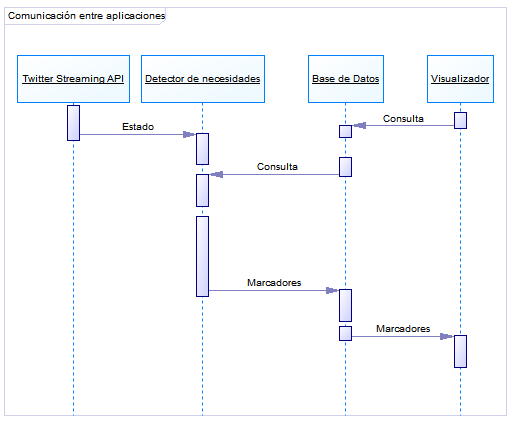
\includegraphics[scale=0.8]{images/ComunicacionFinal.png}
	\caption[Esquema que representa la comunicación entre aplicaciones del sistema detector de necesidades.]{Esquema que representa la comunicación entre aplicaciones del sistema detector de necesidades.\\Fuente: Elaboración Propia, (2016)}
	\label{fig:comunFinal}
\end{figure}

El módulo de detección comienza a recibir datos desde el \textit{stream} de \textit{Twitter} cuando el sistema es activado, luego el módulo de detección realiza consultas a la base de datos buscando si es que el usuario ha hecho ingreso de nuevos términos para filtrar la información entrante. Paralelamente, el módulo de visualización almacena los términos de búsqueda que hayan sido señalados por el usuario. Mientras tanto, el proceso de detección de necesidades continúa. Al concluir el proceso y obtener la respuesta, ésta es utilizada para generar nuevos marcadores, correspondientes a eventos donde se detectaron necesidades, los que pasan a ser almacenados en la base de datos. Periódicamente, el módulo de visualización realiza consultas a la base de datos, por medio de las cuales obtiene todos los nuevos marcadores generados desde la última consulta y los despliega en el mapa de la interfaz.

\subsection{Persistencia}
\label{sec:diseno:persistencia}

Anteriormente, se decidió la implementación de un sistema de persistencia en la aplicación para almacenar la información generada por esta, pero no se ha definido cuál ha de ser el sistema de gestión de base de datos que se ha de utilizar, es por ello que esta sección se presenta el cómo se tomó una decisión con respecto a este punto.

Debido a que se requiere mantener una ventana de datos históricos, se requiere un mecanismo de persistencia o base de datos. Además, los datos han de ser almacenados, al menos durante un tiempo, para que el sistema pueda realizar la generación de estadísiticas con respecto a ellos.

Se consideraron los principales sistemas de bases de datos utilizados y conocidos por el autor, dentro de los cuales se encontraban herramientas relacionales como MySQL, PostgreSQL, SQL Server y MongoDB para el caso de sistemas de gestión de base de datos (DBMS) no relacionales. Dadas las características y las condiciones con las cuales opera el sistema de detección, se requiere de un DBMS con baja latencia en operaciones lectura/escritura. La decisión se tomó en base a como se manejan los datos, pues no se apreció necesidad de implementar una modelo relacional, dado que lo que se requiere es velocidad y no mantener consistencia relacional entre los datos. De esta forma y teniendo en cuenta los resultados presentados en pruebas realizadas por \citep{MongoPerformance}, en las cuales mostró que el tiempo de respuesta (en operaciones de lectura) es significativamente menor en MongoDB que en dos de los DBMS más conocidos como MySQL y PostgreSQL se consideró utilizar este DBMS. Lo anterior, sumado al hecho de la capacidad de escalar de MongoDB reportada en fuentes oficiales o por diversos desarrolladores como \citep{MongoDBScalability} que han compartido sus experiencias en la \textit{Web}, llevaron a decidir que MongoDB debiese ser el sistema de gestión de base de datos que se usase en el sistema.

Para realizar la conexión de MongoDB y el \textit{framework} se utiliza una biblioteca especialmente diseñada para aquello que corresponde a un ORM (Mapeo Objeto-Relacional), denominado \textit{Jongo}\footnote{http://jongo.org/}, para realizar la conversión de objeto Java a JSON y viceversa.

Habiendo resuelto lo anterior, la siguiente problemática que se presenta radica en qué informacion almacenar. Según la definición de la historia de usuario HU-v04 en la que se señalan ``eventos pasados dentro de un intervalo de tiempo", se infiere que ha de guardarse tanto el contenido visible del dato, la clasificación que se le asignó y la fecha en que se identificó, para ello y dado que se seleccionó MongoDB, se especificó un esquema para los documentos de la colección donde sólo resta tener la información correspondiente a la ubicación, por lo que el esquema se definió como se presenta en la Figura \ref{fig:esquemaMarker1} correspondiente a la colección ``Markers".

\begin{figure}[H]
	\centering
	\captionsetup{justification=centering}
	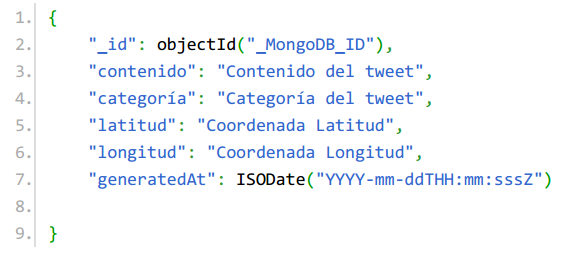
\includegraphics[scale=0.8]{images/Marker1.png}
	\caption[Ejemplo de documento en la colección Markers.]{Ejemplo de documento en la colección Markers.\\Fuente: Elaboración Propia, (2016)}
	\label{fig:esquemaMarker1}
\end{figure}

El primer campo corresponde al ID asignado por \textit{Mongo} para cumplir con la unicidad de los datos, el segundo campo corresponde al contenido textual del \textit{tweet} para ser mostrado junto con el marcador y que el usuario pueda ver desde dónde el sistema asignó aquel \textit{tweet} a una categoría en particular. El tercer campo corresponde al nombre de la etiqueta o categoría asignada al \textit{tweet}, esta asignación está dada por el resultado de la evaluación del clasificador. Los campos cuarto y quinto corresponden a la ubicación geográfica en la que se posiciona el marcador (latitud y longitud), y finalmente, el sexto campo corresponde al momento en que fue creado el marcador para ser utilizado en los diferentes criterios de visualización del sistema (relacionados a la HU-v08).

\subsection{Sistema de procesamiento}
\label{sec:diseno:sistDeProce}

Dado el contexto del funcionamiento del sistema, este ha de entregar respuestas rápidas ante una emergencia. Para ello, y como es descrito en la historia de usuario HU-c00, se requiere de un sistema capaz de procesar eventos en tiempo real que dada la masividad de datos con los que debe lidiar la aplicación, pueda escalar. El problema en este punto es el cómo construir un sistema capaz de identificar necesidades y que posea esta propiedad.

Se consideraron sistemas de procesamiento distribuido \textit{Apache S4}, \textit{Apache Storm} y \textit{Apache Spark}. Estos sistemas tienen la particularidad de poder trabajar con múltiples máquinas. 

Apache S4, pese a su simplicidad, no continuó con su desarrollo luego del año 2013 y nunca tuvo una versión estable ``1.0", razones por las cuales no se consideró como primera opción. Apache Spark, pese a contar con continuos \textit{releases}, una comunidad de desarrolladores no menor y permitir la elaboración de sistemas escalables no era lo que se buscaba en aquel momento como herramienta de desarrollo, pues está orientado al procesamiento por lotes y no en tiempo real. Al momento de consultar con los clientes, estos esperaban que el sistema, internamente, se comportara según el paradigma de procesamiento de \textit{streams}, por medio de operadores dispuestos en un grafo. Por ello finalmente se optó por \textit{Apache Storm}.

\textit{Storm} permite construir sistemas que cumplan con las características de un sistema distribuido, como lo son: escalabilidad (tanto horizontal como vertical) y tolerancia a fallos (como la capacidad de un sistema para realizar correctamente y en todo momento aquello para lo que fue diseñado). Estos sistemas están compuestos por dos tipos de elementos: \textit{Spout} y \textit{Bolt}, descritos en el Capítulo \ref{cap:MarcTeorico}. Al combinar esos elementos se da origen a un grafo dirigido, como el presentado en la Figura \ref{fig:stormBeLike} donde cada elemento de procesamiento (\textit{Bolt}), cumple con una determinada tarea recibiendo como entrada la salida del elemento de nivel anterior.

\subsection{Fuente de datos}
\label{sec:diseno:obtenerDatos}

La historia de usuario HU-c01 refleja desde donde se han de obtener los datos, pero es necesario especificar aún más la forma en la que se obtienen. Como se señaló al momento de definir los alcances de este trabajo, sólo se utiliza \textit{Twitter} como fuente de información, así la unidad básica de información son los \textit{Tweet}.

Existen tres tipos de \textit{streaming endpoints} disponibles para obtener la información, cada uno para un caso de uso particular y son descritos en la Tabla \ref{tab:StreamingEndpoints}.

\begin{table}[H]
\centering
\caption[\textit{Streaming endpoints} de \textit{Twitter}.]{\textit{Streaming endpoints} de \textit{Twitter}.\\Fuente: Elaboración Propia, (2016)}
\label{tab:StreamingEndpoints}
\begin{tabular}{|l|l|}
\hline
Público & \begin{tabular}[c]{@{}l@{}}Stream del que fluye la información pública de Twitter.\\ Casos de uso: Seguimiento de usuarios o tópicos específicos o minería de datos.\end{tabular} \\ \hline
Usuario & Flujo que toda la información correspondiente a un usuario.                                                                                                                       \\ \hline
Sitio   & Versión multi-usuario de la anterior.                                                                                                                                             \\ \hline
\end{tabular}
\end{table}

Para esta aplicación corresponde hacer uso de la API pública. En ésta, a la vez, existen dos puntos de acceso, el acceso público y \textit{firehose}. El acceso público es gratuito y permite el acceso a un 1\% de la información que se genera en tiempo real y para acceder a el basta con crear una aplicación dentro de \textit{Twitter}. En cambio para acceder a \textit{firehose}, el cual permite acceso total a la información, debe comprarse el acceso. Dadas estas condiciones se seleccionó, previo acuerdo con los clientes, el uso de la API pública.

Para hacer uso de la API descrita con anterioridad es necesario obtener cuatro claves de acceso: \textit{Access Token}, \textit{Access Token Secret}, \textit{Consumer Key (API Key)} y \textit{Consumer Secret (API Secret)}. En el \ref{apendice:clavesApi} se incluye más información sobre cómo conseguir estas claves.

\subsection{Términos de búsqueda}
\label{sec:diseno:termBusqueda}

\textit{Twitter4J}\footnote{http://twitter4j.org/}, es una herramienta que permite obtener el flujo de información desde \textit{Twitter} e implementa una forma de filtrado mediante el uso de palabras clave. Sin embargo, la herramienta posee una limitante al momento de realizar modificaciones sobre este filtro, deben instanciarse nuevamente los objetos con los cuales se realiza la conexión a la API de \textit{Twitter}, es decir, volver a instanciar y conectar el \textit{Spout}, eso se traduce en tiempo de procesamiento perdido. Para solucionar este inconveniente se decidió implementar un operador, descrito en la sección \ref{subsec:detectorNecesidades}, el cual está encargado de realizar el filtrado de acuerdo a términos y llevar a cabo las operaciones descritas en la sección \ref{subsubsec:2op} referente a la expansión de la consulta. Sin embargo, un operador como este puede poseer réplicas que operan al mismo tiempo, con esto surge el problema de cómo comunicar y aplicar los nuevos términos de búsqueda y desechar los antiguos.

Para dar solución a esta problemática, se decidió recurrir a la base de datos, almacenar la consulta y asignar un estado para controlar el comportamiento del operador. Así, el esquema en la base de datos queda tal y como se presenta en la Figura \ref{fig:esquemaQuery}, documento de la colección ``Queries".

\begin{figure}[H]
	\centering
	\captionsetup{justification=centering}
	\includegraphics[scale=0.8]{images/Query.png}
	\caption[Ejemplo de documento en la colección queries.]{Ejemplo de documento en la colección queries.\\Fuente: Elaboración Propia, (2016)}
	\label{fig:esquemaQuery}
\end{figure}

La propiedad ``estado" del documento de la colección ``queries" puede tomar dos valores: ``actual" o ``antiguo", reflejando si una consulta se está llevando a cabo o no. Estos valores son asignados por la aplicación responsable de la interfaz, la encargada de recibir los términos de búsqueda por parte del usuario.

Para implementar este operador se desarrollaron dos clases llamadas \textit{CurrentQueryChecker} y \textit{QueryExpander}. La primera, para detectar cuándo y si es que ha cambiado una consulta en la base de datos y la segunda para desarrollar la labor descrita por el algoritmo de expansión presentado en la sección \ref{subsubsec:2op}.

\subsection{Categorización de necesidades}
\label{sec:diseno:categorias}

La definición de las categorías es un punto importante dentro de la construcción de la aplicación. Teóricamente, el tamaño del conjunto de entrenamiento ha de ser mayor o menor dependiendo de la cantidad de clases (categorías). 

Inicialmente, se consideró la taxonomía definida por \citep{TaxonomiaChato}, pero junto al equipo del proyecto FONDEF se estableció que no era conveniente utilizarla, pues presentaba una gran cantidad de categorías demasiado específicas que involucraría un conjunto de datos de entrenamiento muy grande. De manera alternativa se sugirió una clasificación reducida realizada para un proyecto previo (PMI-USA 1204) por \citep{PMIProfes}, junto  a un equipo de psicólogos donde existen cinco categorías bien definidas, basándose en la información obtenida del terremoto de febrero de 2010. Estas categorías antes mencionadas son las siguientes: 

\begin{enumerate}
\item Necesidades básicas: \textit{tweet} que entrege o solicite información sobre serviciós básicos: Agua potable, electricidad y abastecimiento de alimentos.
\item Comunicación: \textit{tweet} que entregue o solicite información sobre alguna localidad.
\item Seguridad: \textit{tweet} que señale un riesgo para la población.
\item Personas: \textit{tweet} que haga referencia al hallazgo o búsqueda de una persona desaparecida.
\item Irrelevante: cualquier otro \textit{tweet}.
\end{enumerate}

Acordando con el equipo, se decidió separar el primer ítem en los tres elementos que lo componen: Agua, alimentos y electricidad. Así, finalmente, se obtienen las siete categorías que se utilizan en el sistema.\\

Los elementos clasificados como ``Irrelevantes" no se muestran en el mapa de eventos, pues hacen referencia a eventos que, pese a haber pasado por todos los operadores anteriormente descritos, no guardan relación con el evento o sus consecuencias. Estos pueden ser \textit{tweets} a etiquetar por expertos \textit{a posteriori} con el objetivo de enriquecer la información del clasificador. Sin embargo, esta tarea está fuera del alcance de este proyecto.

\subsection{Clasificador}
\label{sec:diseno:clasificador}

Se busca generar un clasificador automático capaz de detectar necesidades y lidiar con la jerga nacional. Para ello, según lo descrito por \citep{IRQE} en su libro \textit{Introduction to Information Retrival}, se entrenó un clasificador basado en \textit{Naïve Bayes}, haciendo uso de Mallet, pues presenta mejores resultados en la predicción que RapidMiner y Weka.

La sección \ref{sec:caracteristicasSistema} ya hace referencia a la inconveniencia de utilizar un clasificador estático para el etiquetado de nuevos eventos, al tratarse de un aprendizaje supervisado, donde se requiere de una persona entregue la respuesta esperada para realizar el entrenamiento, no es posible realizar este proceso de manera automática.

Al no poder automatizar el proceso antes señalado se consultó con el equipo del proyecto FONDEF IDeA si es que era factible la implementación de un actualizador manual del clasificador, lo cual fue aceptado.

Segun la metodologia KDD, los pasos que se siguen para construir un nuevo clasificador son los siguientes:

Los datos son seleccionados por el usuario, estos datos se agruparan en un archivo de texto, un archivo CSV en el cual los elementos se separaran utilizando el caracter punto y coma (;). El formato que se utiliza para el archivo de entrada se muetra en la Figura \ref{fig:formatoFig} , así cualquier archivo que cumpla con el formato permite la creación de un nuevo modelo clasificador.

\begin{figure}[H]
	\centering
	\captionsetup{justification=centering}
	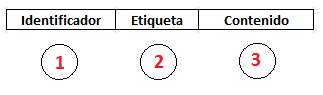
\includegraphics[scale=0.8]{images/FormatoArchivoEntrada.png}
	\caption[Formato archivo de entrada.]{Formato archivo de entrada.\\Fuente: Elaboración Propia, (2016)}
	\label{fig:formatoFig}
\end{figure}

\begin{enumerate}
\item Corresponde a un identificador arbitrario, pero necesario para la herramienta de clasificación Mallet.
\item Corresponde a la etiqueta que categoriza al contenido.
\item Contenido del \textit{tweet} propiamente tal.
\end{enumerate}

El preprocesamiento y transformación de los datos se realiza utilizando los operadores de transformación (normalizador de texto, eliminación de \textit{stopwords} y proceso de \textit{stemming}), presentados en la sección \ref{subsec:detectorNecesidades}.

Teniendo en consideración que se utilizan dos módulos distintos, donde en uno se construye el clasificador y es utilizado en el otro módulo, surge el problema de cómo realizar la comunicación entre ellos. Para solucionar este inconveniente se utiliza una carpeta compartida por ambas aplicaciones. En el caso de sistemas Unix se utiliza el directorio $/opt/DeNe$, mientras que para Windows se utiliza $C:/DeNe/$. En estos directorios se almacena un fichero con el clasificador serializado.

\begin{figure}[H]
	\centering
	\captionsetup{justification=centering}
	
\includegraphics[scale=0.8]{images/ClasifierDene.png}
	\caption[Fichero clasificador en $c:/DeNe/$.]{Fichero clasificador en $C:/DeNe/$.\\Fuente: Elaboración Propia, (2016)}
	\label{fig:TopologiaGeneral}
\end{figure}

Cada vez que se actualice el clasificador se contrasta el nuevo con el ya existente por medio de lós indicadores precisión, \textit{recall} y \textit{F-1 Score}, definidos en la sección \ref{subsec:MineriaTexto}. En el caso de encontrar mejores indicadores en el primero, se reemplaza en las carpetas antes mencionadas, según el sistema operativo de la máquina que se esté utilizando. En caso contrario, se mantiene el anterior. En todos los escenarios se le da a conocer al usuario los indicadores de ambos clasificadores.

\subsection{Interfaz web}
\label{sec:diseno:interfaz}

Teniendo en consideración la característica del desarrollo de esta aplicación como un proyecto ágil con un mínimo de personal de desarrollo se requería de un \textit{framework} que contribuyera a acelerar la construcción de la aplicación. Tras considerar las alternativas más conocidas como \textit{Spring}, \textit{Hibernate} o \textit{JSF} que tienen una curva de aprendizaje elevada, se optó por utilizar un cuarto \textit{framework} que aunque desconocido, promete una simplicidad en su uso. \textit{Play Framework}\footnote{https://www.playframework.com/}, construido haciendo uso de Scala y Java permite construir aplicaciones ligeras (tamaño en disco), sin estado (no guarda configuraciones de una sesión para ser utilizadas luego) y por defecto RESTful, ideal para la comunicación entre aplicaciones. Este \textit{framework} sigue el patrón de arquitectura Modelo-Vista-Controlador (MVC) y cuenta con un compilador en tiempo real (compila y realiza el despliegue de la aplicación cuando detecta un cambio en el código), lo que agiliza en gran medida el desarrollo, pues al automatizar este proceso mantiene la atención en lo que se está desarrollando.

Para visualizar los puntos encontrados por el detector de necesidades se decidió utilizar la API de \textit{Google Maps} la que permite la colocación de los denominados ``marcadores" en un punto específico del mapa y asociar a ellos algún tipo de información. Así, aunque el funcionamiento interno esté dirigido por \textit{Play}, la principal funcionalidad del sistema, mostrar el mapa con sus marcadores, es implementada por medio de Javascript haciendo uso de esta API.

Los marcadores, ya ubicados en el mapa, tienen asociado un cuadro de texto dentro del cual refleja el la categoría a la que pertenece y el \textit{tweet} original que lo generó. La Figura \ref{fig:EjemploMarker} presenta un ejemplo de este funcionamiento en la interfaz \textit{Web}. La visualización del contenido del \textit{tweet} tiene como objetivo permitir decidir, en última instancia, al usuario si ha sido correctamente clasificado.

\begin{figure}[H]
	\centering
	\captionsetup{justification=centering}
	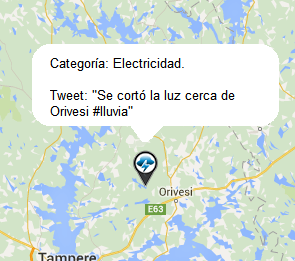
\includegraphics[scale=0.8]{images/EjemploMarker.png}
	\caption[Ejemplo de marcador en el mapa con su categorización y \textit{tweet} que lo generó.]{Ejemplo de marcador en el mapa con su categorización y \textit{tweet} que lo generó.\\Fuente: Elaboración Propia, (2016)}
	\label{fig:EjemploMarker}
\end{figure}

Según lo solicitado en la historia de usuario HU-v02 se prepararon dos tipos de filtros a la interfaz para la visualización de eventos en el mapa: El primero considera el agrupamiento o \textit{clustering} de marcadores, mientras que el segundo considera el tipo de marcador o marcadores que se desean visualizar.

Para el caso del agrupamiento se definieron tres modos de funcionamiento los cuales se describen a continuación:

\begin{enumerate}
\item No agrupar: Mostrar todos los marcadores que correspondan en el mapa de acuerdo al punto geográfico que corresponda en su definición.
\item Agrupar por distancia: Define una grilla invisible en el mapa donde los elementos que calcen en una cudrícula son agregados a un \textit{cluster} y visualizados como tal.
\item Agrupar por categoría: De igual forma que el agrupamiento por distancia, pero sólo agrega elementos que comparan categoría.
\end{enumerate}

La Figura \ref{fig:EjemploAmbosClusters} presentan un ejemplo de ambos tipos de agrupamiento especial, respectivamente por distancia y categoría.

\begin{figure}[H]
\centering
\captionsetup{justification=centering}
\subfloat[Cluster distancias.]{\centering\label{fig:mdleft}{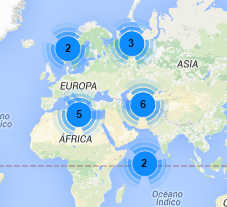
\includegraphics[width=0.45\textwidth]{images/EjemploCluster.png}}}\hfill
\subfloat[Cluster categoría.]{\centering\label{fig:mdleft}{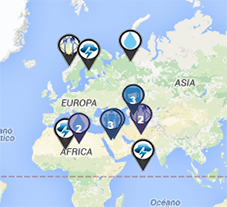
\includegraphics[width=0.45\textwidth]{images/ClusterCategoria.png}}}
\caption[Ejemplos de agrupamiento basados en distancia y categorías.]{Ejemplos de agrupamiento basados en distancia y categorías.\\Fuente: Elaboración Propia, (2016)}
\label{fig:EjemploAmbosClusters}
\end{figure}

Para el segundo caso sólo se definieron dos reglas de funcionamiento las cuales se describen a continuación:

\begin{enumerate}
\item Mostrar todos: Muestra elementos de todas las categorias existentes.
\item Mostrar categoría: Para cada categoría mostrar sólo los elementos de aquella categoría. 
\end{enumerate}

Al combinar ambos tipos de filtros se tienen potencialmente seis modos de funcionamiento, pero considerando las categorías descritas en al sección \ref{sec:diseno:categorias} ese número se expande a veintidós modos de funcionamiento del visualizador.

\section{Implementación del sistema}
\label{sec:implementacion}

En la presente sección se detalla el proceso de implementación de la solución diseñada. Para ello se trabaja en paralelo en el desarrollo de ambos modulos: \textit{front-end} y \textit{back-end} bajo la metodologia XP, donde se generan versiones sucesivas de la solución, las cuales evolucionan de acuerdo a los requermientos del cliente.

\subsection{\textit{Front-end}}
\label{subsec:imp:visualizador}

La implementación del visualizador de eventos se realizó haciendo uso del \textit{framework} de Java \textit{Play}, el cual por defecto crea aplicaciones que siguen el patrón de diseño MVC, por lo tanto se tienen tres niveles dentro de la aplicación:

\begin{itemize}
\item Modelo: donde están los elementos que permiten interactuar con la base de datos. 
\item Controlador: presentando los métodos de reacción ante los eventos detonados en el nivel de presentación.
\item Vista o presentación: muestra las interfaces \textit{Web} diseñadas para que el usuario interactúe con el sistema.
\end{itemize}

\subsubsection*{Filtrado de marcadores}
\label{subsubsec:filtradoMarcadores}

Dentro del nivel de presentación se encuentra el mapa proporcionado por la API de Google Maps como se mencionó en la sección \ref{sec:diseno:interfaz}. Allí se señaló que existen filtros para la visualización de eventos de manera que la presentación de estos se apegue a las necesidades del usuario. Para implementar estos filtros, internamente la aplicación hace uso de $n + 1$ \textit{clusters}, donde $n$ corresponde al número de categorías y el cluster extra es para agruparlos a todos. Así, en el caso de querer ver los eventos agrupados, y dependiendo si se quiere o no agruparlos discriminando su categoría, se llenan los \textit{clusters} pertenecientes a la visualización general o a la visualización por categoría. Para el caso de querer mostrar sólo una categoría en particular, sólo se permite que los \textit{cluster} se llenen con los elementos de la categoría seleccionada. El Algoritmo \ref{alg:filtroMarcadores} presenta lo anteriormente descrito para facilitar la comprensión de la lógica interna de los filtros presentados.\\

\begin{algorithm}[H]\setstretch{1.5}
	\begin{algorithmic}[numeracion_lineas]
		\REQUIRE Tipo de agrupamiento $A$.
		\REQUIRE Discriminador de categoría $K$.
		\REQUIRE Marcadores $M$.
		\STATE Lista de marcadores $L$.
		\STATE \textit{Clusters} de marcadores $C = \{c_{0}, \dots, c_{n+1} \}$.
		\FOR{cada $m_{i}$ perteneciente a $M$}
			\IF{la categoría de $m_{i}$ no es ``irrelevante" y la categoría de $m_{i}$ es igual a $K$}
				\STATE añadir el marcador a $L$.
			\ELSIF{$K$ es ``todas las categorías"}
				\STATE añadir el marcador a $L$.
			\ENDIF
		\ENDFOR
		\IF{$A$ es ``no agrupar"}
			\FOR{cada $l_{i}$ perteneciente a $L$}
				\STATE posicionar $l_{i}$ en el mapa.
			\ENDFOR
		\ELSIF{$A$ es ``agrupar todos"}
			\FOR{cada $l_{i}$ perteneciente a $L$}
				\STATE añadir $l_{i}$ al clister $c_{0}$.
			\ENDFOR
			\STATE posicionar $c_{0}$ en el mapa.
		\ELSE
			\FOR{cada $l_{i}$ perteneciente a $L$}
				\STATE añadir $l_{i}$ al cluster $c_{i+1}$
			\ENDFOR
			\FOR{cada $c_{i}$ perteneciente a $C - \{c_{0}\}$}
				\STATE añadir $l_{i}$ al cluster $c_{i}$
			\ENDFOR
		\ENDIF
	\end{algorithmic}
	\caption{Algoritmo de utilización de filtros}
	\label{alg:filtroMarcadores}
\end{algorithm}\vphantom\\

Para realizar la selección del intervalo mencionado en la HU-v04 se solicitó, por parte del equipo FONDEF IDeA, el uso de una línea de tiempo con intervalo deslizante que, además, mostrase la cantidad de eventos detectados por fecha por medio de un histograma. Para ello se utilizó inicialmente \textit{JDateRangeSlider}, de la biblioteca Javascript \textit{JQRangeSlider}\footnote{http://ghusse.github.io/jQRangeSlider/}, \citep{JQRangeSlider}. Esta biblioteca era suficiente para seleccionar el intervalo de fechas y detectar cambios producidos en la línea de tiempo para actualizar los valores, mas no permite la implementación de un histograma externo.

\begin{figure}[H]
	\centering
	\captionsetup{justification=centering}
	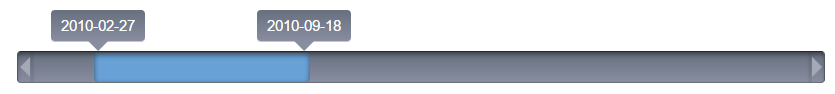
\includegraphics[scale=0.6]{images/JDateRangeSlider.png}
	\caption[Selectorde fechas JDateRangeSlider.]{Selectorde fechas JDateRangeSlider.\\Fuente: \citep{JQRangeSlider}}
	\label{fig:JQRangeSlider}
\end{figure}

Para lograr implementar ambas funcionalidades, línea de tiempo e histograma, se utilizó una biblioteca Javascript distinta. La Figura \ref{fig:HistogramaFinal} presenta la implementación utilizando \textit{HighCharts}, \citep{Highcharts}. Esta biblioteca, al contrario de \textit{JQRangeSlider}, no permitía capturar los cambios en el histograma para reaccionar cuando se produjese un cambio en él. Para solucionar este inconveniente se implementó una función Javascript que recogiese los valores actuales del intervalo y arrojase un evento cuando se produjece un cambio. Este evento se asoció al eje x de la línea temporal. De esta manera, cada vez que se modifiquen los valores del eje se dispare un nuevo evento, el que pasa a ser capturado y produce la actualización de los marcadores del mapa. La implementación del disparador de este evento es descrito en la Figura \ref{fig:implementacionCambiosEnEje}.

\begin{figure}[H]
	\centering
	\captionsetup{justification=centering}
	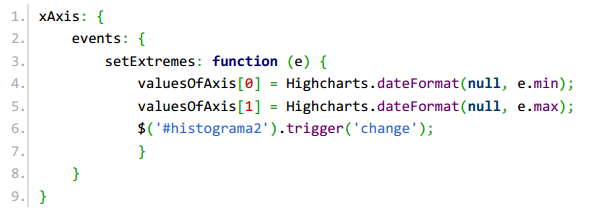
\includegraphics[scale=0.8]{images/onChangeEventTimeline.png}
	\caption[Implementación de evento de detección de cambios en la línea temporal.]{Implementación de evento de detección de cambios en la línea temporal.\\Fuente: Elaboración Propia, (2016)}
	\label{fig:implementacionCambiosEnEje}
\end{figure}

Inicialmente este histograma sólo está disponible en inglés, pero permite cambiar todas sus etiquetas manualmente. Así, para mejorar la usabilidad de la aplicación se modificaron todos los textos para estuviesen en español. El resultado de esta modificación es presentado en la Figura \ref{fig:HistogramaFinal}.

\begin{figure}[H]
	\centering
	\captionsetup{justification=centering}
	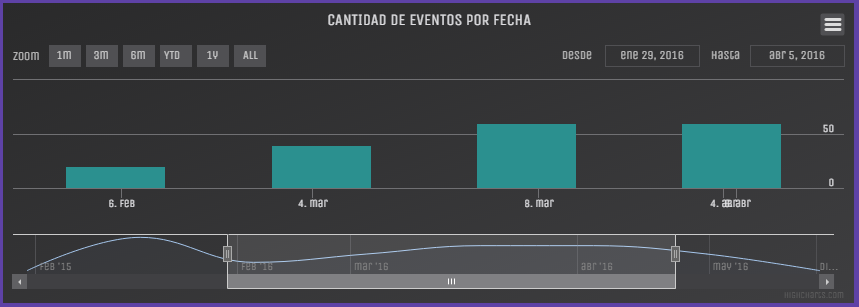
\includegraphics[scale=0.6]{images/Histograma.png}
	\caption[Selector de fechas presente en la aplicación.]{Selector de fechas presente en la aplicación.\\Fuente: Elaboración Propia, (2016)}
	\label{fig:HistogramaFinal}
\end{figure}

Tras la selección de intervalo dentro del cual se desea que el sistema muestre los estados recibidos, se realiza una consulta del tipo POST con parámetros fecha inicial y final, para obtener una lista con todos los marcadores encontrados en ese rango.

Los iconos correspondientes a las categorías que soporta el sistema se definieron mediante la combinación de dos imágenes para cada categoría: un marcador de mapa, similar a los definidos en la API de Google Maps y una que sugiriera al usuario la categoría a la que hace referenciar. Los diseños finales son presentados en la Figura \ref{fig:categoriasFig}

\begin{figure}[H]
\centering
\subfloat[Categoría agua.]{
	\makebox[4cm][c]{
		\label{fig:mdleft}{
			
\includegraphics[width=1.5cm]{images/categorias/agua.png}
		}
	}
}\hfill
\subfloat[Categoría alimento.]{
	\makebox[4cm][c]{
		\label{fig:mdleft}{
			
\includegraphics[width=1.5cm]{images/categorias/alimento.png}
		}
	}
}\hfill
\subfloat[Categoría electricidad.]{
	\makebox[4cm][c]{
		\label{fig:mdright}{
			
\includegraphics[width=1.5cm]{images/categorias/electricidad.png}
		}
	}
}\hfill
\vfill
\subfloat[Categoría comunicación]{
	\makebox[4cm][c]{
		\label{fig:mdleft}{
			
\includegraphics[width=1.5cm]{images/categorias/comunicacion.png}
		}
	}
}\hfill
\subfloat[Categoría personas.]{
	\makebox[4cm][c]{
		\label{fig:mdleft}{
			
\includegraphics[width=1.5cm]{images/categorias/personas.png}
		}
	}
}\hfill
\subfloat[Categoría seguridad.]{
	\makebox[4cm][c]{
		\label{fig:mdright}{
			
\includegraphics[width=1.5cm]{images/categorias/seguridad.png}
		}
	}
}\hfill
\caption[Categorías para marcadores.]{Iconos de categorías para marcadores.\\Fuente: Elaboración Propia, (2016)}
\label{fig:categoriasFig}
\end{figure}

Además, se consideró apropiado diseñar un icono que representara la densidad de marcadores al momento de realizar el agrupamiento por categorías descrito en esta sección, para ello y siguiendo la combinación de colores utilizada por la biblioteca \textit{MarkerClusterer} donde se muestra un cluster azul cuando es un cluster pequeño; amarillo para uno medio y rojo para uno grande, \citep{MarkerClusterer}. La definición de estos colores es descrita a continuación:

\begin{itemize}
\item Azul: De dos a diez elementos.
\item Amarillo: De once a cien elementos amarillo.
\item Rojo: Desde cien elementos.
\end{itemize}

Se prepararon tres iconos adicionales a cada categoría para reemplazar los íconos por defecto de la biblioteca, las que pueden verse en las Figuras \ref{fig:clusterAgua}. a la \ref{fig:clusterseguridad}.

\begin{figure}[H]
\centering
\subfloat[Cluster pequeño.]{
	\makebox[4cm][c]{
		\label{fig:mdleft}{
			
\includegraphics[width=1.5cm]{images/categorias/aguaS.png}
		}
	}
}\hfill
\subfloat[Cluster medio.]{
	\makebox[4cm][c]{
		\label{fig:mdleft}{
			
\includegraphics[width=1.5cm]{images/categorias/aguaM.png}
		}
	}
}\hfill
\subfloat[Cluster grande.]{
	\makebox[4cm][c]{
		\label{fig:mdright}{
			
\includegraphics[width=1.5cm]{images/categorias/aguaL.png}
		}
	}
}
\caption[Iconos de cluster para categoría agua.]{Iconos de cluster para categoría agua.\\Fuente: Elaboración Propia, (2016)}
\label{fig:clusterAgua}
\end{figure}

\begin{figure}[H]
\centering
\subfloat[Cluster pequeño.]{
	\makebox[4cm][c]{
		\label{fig:mdleft}{
			
\includegraphics[width=1.5cm]{images/categorias/alimentoS.png}
		}
	}
}\hfill
\subfloat[Cluster medio.]{
	\makebox[4cm][c]{
		\label{fig:mdleft}{
			
\includegraphics[width=1.5cm]{images/categorias/alimentoM.png}
		}
	}
}\hfill
\subfloat[Cluster grande.]{
	\makebox[4cm][c]{
		\label{fig:mdright}{
			
\includegraphics[width=1.5cm]{images/categorias/alimentoL.png}
		}
	}
}
\caption[Iconos de cluster para categoría alimento.]{Iconos de cluster para categoría alimento.\\Fuente: Elaboración Propia, (2016)}
\label{fig:clusteralimento}
\end{figure}

\begin{figure}[H]
\centering
\subfloat[Cluster pequeño.]{
	\makebox[4cm][c]{
		\label{fig:mdleft}{
			
\includegraphics[width=1.5cm]{images/categorias/electricidadS.png}
		}
	}
}\hfill
\subfloat[Cluster medio.]{
	\makebox[4cm][c]{
		\label{fig:mdleft}{
			
\includegraphics[width=1.5cm]{images/categorias/electricidadM.png}
		}
	}
}\hfill
\subfloat[Cluster grande.]{
	\makebox[4cm][c]{
		\label{fig:mdright}{
			
\includegraphics[width=1.5cm]{images/categorias/electricidadL.png}
		}
	}
}
\caption[Iconos de cluster para categoría electricidad.]{Iconos de cluster para categoría electricidad.\\Fuente: Elaboración Propia, (2016)}
\label{fig:clusterelectricidad}
\end{figure}

\begin{figure}[H]
\centering
\subfloat[Cluster pequeño.]{
	\makebox[4cm][c]{
		\label{fig:mdleft}{
			
\includegraphics[width=1.5cm]{images/categorias/comunicacionS.png}
		}
	}
}\hfill
\subfloat[Cluster medio.]{
	\makebox[4cm][c]{
		\label{fig:mdleft}{
			
\includegraphics[width=1.5cm]{images/categorias/comunicacionL.png}
		}
	}
}\hfill
\subfloat[Cluster grande.]{
	\makebox[4cm][c]{
		\label{fig:mdright}{
			
\includegraphics[width=1.5cm]{images/categorias/comunicacionL.png}
		}
	}
}
\caption[Iconos de cluster para categoría comunicación.]{Iconos de cluster para categoría comunicación.\\Fuente: Elaboración Propia, (2016)}
\label{fig:clustercomunicacion}
\end{figure}

\begin{figure}[H]
\centering
\subfloat[Cluster pequeño.]{
	\makebox[4cm][c]{
		\label{fig:cluster}{
			
\includegraphics[width=1.5cm]{images/categorias/personasS.png}
		}
	}
}\hfill
\subfloat[Cluster medio.]{
	\makebox[4cm][c]{
		\label{fig:mdleft}{
			
\includegraphics[width=1.5cm]{images/categorias/personasM.png}
		}
	}
}\hfill
\subfloat[Cluster grande.]{
	\makebox[4cm][c]{
		\label{fig:mdright}{
			
\includegraphics[width=1.5cm]{images/categorias/personasL.png}
		}
	}
}
\caption[Iconos de cluster para categoría personas.]{Iconos de cluster para categoría personas.\\Fuente: Elaboración Propia, (2016)}
\label{fig:clusterpersonas}
\end{figure}

\begin{figure}[H]
\centering
\subfloat[Cluster pequeño.]{
	\makebox[4cm][c]{
		\label{fig:mdleft}{
			
\includegraphics[width=1.5cm]{images/categorias/seguridadS.png}
		}
	}
}\hfill
\subfloat[Cluster medio.]{
	\makebox[4cm][c]{
		\label{fig:mdleft}{
			
\includegraphics[width=1.5cm]{images/categorias/seguridadM.png}
		}
	}
}\hfill
\subfloat[Cluster grande.]{
	\makebox[4cm][c]{
		\label{fig:mdright}{
			
\includegraphics[width=1.5cm]{images/categorias/seguridadL.png}
		}
	}
}
\caption[Iconos de cluster para categoría seguridad.]{Iconos de cluster para categoría seguridad.\\Fuente: Elaboración Propia, (2016)}
\label{fig:clusterseguridad}
\end{figure}

Dado que se solicitó que la interfaz no se recargue cada vez que se produzca un cambio dado por un nuevo evento detectado o la modificación en el intervalo de visualización, se utilizaron las tecnologías Javascript y AJAX para capturar los cambios en la línea temporal al momento de su ocurrencia, descrita en esta sección. Cada vez que se detecte un cambio, se elimina todo marcador del mapa y se reubican en todos los que cumplan con los parámetros de búsqueda sin necesidad de refrescar la página completa.

\subsubsection*{Estadísticas de procesamiento}
\label{subsubsec:estadisticasdeproc}

Específicamente se solicitaron tres tipos de estadísticas que han de ser mostradas por consulta, estas se definen a continuación:

\begin{enumerate}
\item Cantidad de eventos detectados, es decir, \textit{tweets} que fueron clasificados.
\item Cantidad de usuarios distintos identificados en aquellos eventos.
\item Cantidad total de \textit{tweets} que han pasado por el sistema desde el inicio de la consulta actual.
\end{enumerate}

Para cumplir lo solicitado se necesitaba añadir elementos no considerados en la base de datos; hace falta conocer al usuario y contar los \textit{tweets} ingresados desde \textit{Twitter4J}.

Para completar esta historia se realizaron modificaciones al esquema previamente definido en la sección \ref{sec:diseno:persistencia}, este de por sí era suficiente para cumplir con la estadística número uno, pero incapaz de realizar las otras dos. Para la segunda estadística se consideró que bastaba con guardar al usuario junto con la colección de marcadores. De acuerdo a \citep{TwitterAgreement} en su sección F. \textit{Be a Good Partner to Twitter}, se insta a los desarrolladores que almacenen contenido \textit{offline} de \textit{Twitter}, a almacenar sólo el ID del usuario o del \textit{tweet}, por ello y siguiendo estos lineamientos se agrega el campo ``userID" al esquema marcadores, pasando a quedar como se aprecia en la Figura \ref{fig:esquemaMarker2}.

\begin{figure}[H]
	\centering
	\captionsetup{justification=centering}
	\includegraphics[scale=0.8]{images/Marker2.png}
	\caption[Ejemplo de documento en la colección Markers.]{Ejemplo de documento en la colección Markers.\\Fuente: Elaboración Propia, (2016)}
	\label{fig:esquemaMarker2}
\end{figure}

Para la tercera estadística la colección de marcadores no sería útil, pues no refleja la cantidad de tweets procesados, para ello es necesario implementar una tercera colección de documentos en la base de datos y almacenarlos antes de la aplicación de cualquier tipo de filtro. Esta colección tiene el esquema presente en la Figura \ref{fig:esquemaTweet}.

\begin{figure}[H]
	\centering
	\captionsetup{justification=centering}
	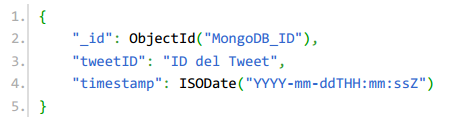
\includegraphics[scale=0.8]{images/status.png}
	\caption[Ejemplo de documento en la colección Status.]{Ejemplo de documento en la colección Status.\\Fuente: Elaboración Propia, (2016)}
	\label{fig:esquemaTweet}
\end{figure}

Al almacenar sólo el identificador del \textit{tweet} no viola las políticas de uso descritas de \textit{Twitter}, sólo es necesaria la fecha para realizar la estadística. En general la obtención de estas estadísticas se realiza utilizando el Algoritmo \ref{alg:estadisticas}.\\

\begin{algorithm}[H]\setstretch{1.5}
	\begin{algorithmic}[numeracion_lineas]
		\REQUIRE Colección $c$ 
		\REQUIRE Fecha de la consulta actual $f$ 
		\ENSURE Contador de eventos $counter$  
		\STATE $counter = 0$
		\FOR{Documento $d_{i}$ en la colección $c$}
			\IF{ fecha de $d_{i}$ es posterior a $f$}
				\STATE $counter = counter + 1$
			\ENDIF	
		\ENDFOR
		\RETURN $counter$
	\end{algorithmic}
	\caption{Algoritmo de generación de primera y tercera estadística.}
	\label{alg:estadisticas}
\end{algorithm}\vphantom\\

Este algoritmo, como se mencionó, es de uso general y permite cumplir tanto la primera como la tercera estadística, para el caso de la segunda se requiere una modificación, pues se solicitó conocer los usuarios diferentes, el Algoritmo \ref{alg:estadisticas2} presenta el algoritmo modificado para la segunda estadística.\\

\begin{algorithm}[H]\setstretch{1.5}
	\begin{algorithmic}[numeracion_lineas]
		\REQUIRE Colección $c$ 
		\REQUIRE Fecha de la consulta actual $f$ 
		\ENSURE Lista de usuarios vacía $list$  
		\FOR{Documento $d_{i}$ en la colección $c$}
			\IF{ fecha de $d_{i}$ es posterior a $f$}
				\IF{ID del usuario de $d_{i}$ no está en $list$ o $list$ es vacía}
					\STATE Añadir $d_{i}$ a $list$
				\ENDIF
			\ENDIF	
		\ENDFOR
		\RETURN Cantidad de elementos en $list$
	\end{algorithmic}
	\caption{Algoritmo de generación de segunda estadísticas.}
	\label{alg:estadisticas2}
\end{algorithm}\vphantom\\

Para mostrar las estadísticas es necesario comunicar los datos al \textit{front-end} de la aplicación, para lo cual se utiliza el mismo principio utilizado para la actualización de los marcadores, en donde cada cierto tiempo se consulta a la base de datos por nuevos marcadores. Para el caso de las estadísticas se implementó un servicio de consulta del tipo GET para obtener, mediante AJAX, el valor del resultado de la implementación de los algoritmos expuestos anteriormente.

\subsubsection*{Configuración}
\label{subsubsec:config}

La necesidad de un segmento de configuración nace producto de la HU-v01. El visualizador de eventos tiene dos maneras de comportarse:

\begin{itemize}
\item Modo tiempo real: Cuando el sistema esté en funcionamiento y cada cierto tiempo, $t_{1}$, se actualizan los marcadores de los nuevos eventos y estos se muestran durante un tiempo, $t_{2}$.
\item Modo línea de tiempo: Funcionamiento basado en lo descrito en HU-v04.
\end{itemize}

Los tiempos $t_{1}$ y $t_{2}$ inicialmente fueron decididos de manera arbitraria, pero al mostrar su funcionamiento se sugirió que estos parámetros pudiesen ser definidos por el usuario. Por ello, se implementó una sección de configuración dentro de la aplicación de visualización para permitir la definición de estos valores. La importancia de la definición de estos valores viene dada por las necesidades del usuario, pero traen consecuencias al sistema.

Para el caso del tiempo $t_{1}$, un menor $t_{1}$ implica que se realizan más consultas al sistemas, pese a esto, es adecuado un valor pequeño cuando se encuentre en operación y el sistema de detección esté generando contenido constantemente. Para la operación en periodos normales, es decir, cuando no esté ocurriendo un evento del tipo desastre, la generación de eventos es muy baja o nula, en esas ocaciones es recomentable un $t_{1}$ elevado.

Para el caso del tiempo $t_{2}$, este está dado por el tiempo que el usuario estime que un evento se encuentra vigente. El valor de t2 no afecta de gran manera al sistema, pues sólo tiene fines visuales, descartando eventos que no cumplan con la ventana de tiempo $Tiempo actual - tiempo de creación \geq t_{2}$, a mayor $t_{2}$, mayor es la ventana de tiempo en la que un evento se considera vigente.

\subsection{Back-end}
\label{subsec:detectorNecesidades}

El detector de necesidades se implementa utilizando un motor de procesamiento de \textit{stream}, en este caso \textit{Storm}. La implementación de \textit{Storm} requiere de la definición de una topología de grafo compuesta por operadores que realizan tareas y comparten eventos. Para implementar el detector se requirió de la construcción de operadores especializados capaces de realizar alguna de las tareas necesarias para detectar las necesidades expresadas en el texto. A continuación se presenta la construcción de estos operadores.

\subsubsection*{Operador fuente de datos}
\label{subsubseC:EntradaDeDatos}

Este operador es el encargado de conectarse a la fuente de datos, en este caso la API de \textit{Twitter}, y comunicar los eventos resto del sistema de procesamiento de \textit{stream}. En el caso particular de \textit{Storm}, este operador corresponde a un \textit{Spout}.

Conociendo desde donde se obtiene la información y teniendo acceso a ella resta conocer cómo realizar la conexión. Para ello se decidió utilizar \textit{Twitter4J}, una biblioteca no oficial de Java para las API de \textit{Twitter}. Para su funcionamiento sólo requiere del uso de Java en su versión 5 o superior.

La implementación de lo anteriormente descrito se realiza utilizando una instancia del objeto \textit{TwitterStream}, el cual captura el flujo público de \textit{Twitter}, almacenando cada \textit{tweet} recibido en una cola. Con esto en mente se construyó el primer operador del sistema correspondiente al \textit{Spout} que surte de datos al sistema.

\begin{figure}[H]
	\centering
	\captionsetup{justification=centering}
	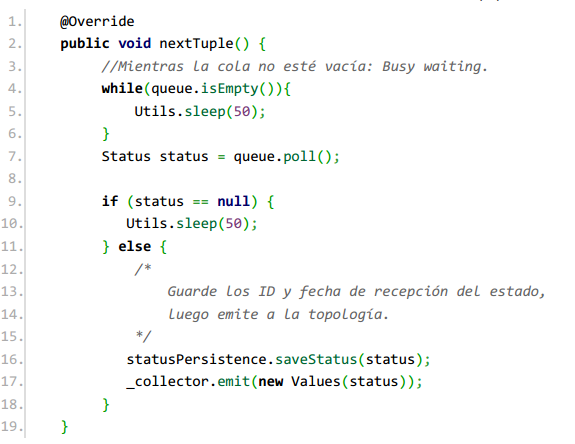
\includegraphics[scale=0.8]{images/TwitterSpout.png}
	\caption[Implementación del \textit{Spout} del sistema.]{Implementación del \textit{Spout} del sistema.\\Fuente: Elaboración Propia, (2016)}
	\label{fig:TwitterSpout}
\end{figure}

Considerando lo recién expuesto en la Figura \ref{fig:TwitterSpout} muestra cómo los estados son emitidos por el \textit{spout} al sistema basándose en la cola (\textit{queue}) para manejar lo que llega desde el \textit{stream}. Al ser llamado por parte de \textit{Storm}, el método \textit{nextTuple} espera a que la cola de eventos no esté vacía y cuando esto se cumple toma un \textit{tweet} (\textit{status}) y lo emite al sistema, no sin antes almacenar su ``tweetID" con fines estadísticos.

\subsubsection*{Operador idioma}
\label{subsubsec:1op}

El presente trabajo se enfoca en la detección de necesidades en español. De acuerdo a \citep{TwitterActiveUsers}, existen actualmente 310 millones de usuarios activos en \textit{Twitter} (a enero del 2016), de los cuales 65 millones pertenecen a los Estados Unidos, cuyo idioma oficial es el inglés, según \citep{TwitterStats1}. Se estima que este año, en latinoamérica, Brasil, cuyo idioma oficial es el portugués, alcance los 15 millones de usuarios según \citep{TwitterStats2}, sin considerar paises árabes o asiáticos podemos deducir que al menos un 30\% de los usuarios activos de \textit{Twitter} hablan idiomas distintos al español. Dado que el sistema está pensado para operar dentro de Chile donde el idioma oficial es el español, se hace necesario filtrar todos aquellos \textit{tweets} que estén escritos en un idioma distinto al este. Este operador de filtrado debe ser ubicado luego del \textit{spout}, dado que todo evento que no cumpla esta condición no es de interés para la aplicación, de esta manera se evita procesar eventos que no aportan información para el sistema.

\citep{languageDetector} desarrolló un módulo capaz de detectar con éxito 49 idiomas dentro de un texto con un 99.8\% de precisión haciendo uso de un clasificador \textit{Naïve Bayes}. Sin embargo, la ejecución de este detector es costosa, razón por la cual se decidió implementar la seleccion de idioma con un mecanismo de filtrado basado en los metadatos del \textit{tweet}, donde, precisamente uno corresponde al idioma de éste. Si bien no es del todo preciso, el costo de selección es bajo y en pruebas realizadas se demostró que es capaz de filtrar de manera correcta un alto porcentaje de los mensajes.

La Figura \ref{fig:operadorIdioma} presenta el código de la implementación de este \textit{Bolt}, correspondiente a su método \textit{execute}, llamado cada vez que \textit{Storm} requiere hacer uso del operador. El operador obtiene la tupla entrante y revisa que el valor del campo ``lang" corresponda al idioma en cuestión, en este caso, el español. Aunque simple, el operador filtra un gran número de estados, dado que según lo dicho anteriormente, la mayoría de los usuarios de \textit{Twitter} no son hispano-hablantes. 

\begin{figure}[H]
	\centering
	\captionsetup{justification=centering}
	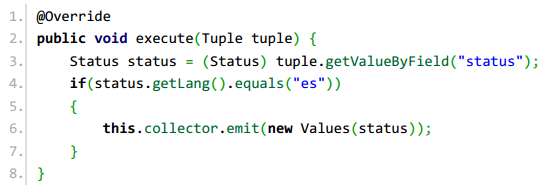
\includegraphics[scale=0.8]{images/LanguageBoltExecute.png}
	\caption[Implementación del método \textit{execute} del \textit{bolt} de idioma.]{Implementación del método \textit{execute} del \textit{bolt} de idioma.\\Fuente: Elaboración Propia, (2016)}
	\label{fig:operadorIdioma}
\end{figure}

\subsubsection*{Operador filtro de consultas}
\label{subsubsec:2op}

El segundo nivel de operadores consiste en un segundo filtro, en este caso, los filtros introducidos por el usuario para discriminar \textit{tweets} según su contenido. Esto busca centrar la atención del sistema en los términos importantes para el usuario. De esta forma la cantidad de datos que ingresa al sistema puede verse reducida aún más en función de qué términos se hayan sido especificados.

Adicionalmente a lo anterior se encuentra que la historia HU-c02. Esta historia menciona la necesidad de incrementar los términos de búsqueda para enriquecerla y así incrementar la cantidad de \textit{tweets} relacionados al evento. Para realizar esto se consideró una práctica del procesamiento de lenguaje natural como es la denominada \textit{Query Expansion} (QE). Según lo descrito por \citep{IRQE} son técnicas comunes al utilizar QE la búsqueda de sinónimos (uso de diccionarios priviamente establecidos), diccionarios basados en la minería de los elementos previamente hayados, creación de diccionadios basados en la co-ocurrencia de términos, es decir, términos que suelen venir juntos o un vocabulario mantenido por editores humanos. Para este trabajo sólo se consideran las dos primeras: Búsqueda por diccionario de sinónimos y una implementación que encuentra los términos más frecuentes dentro de los resultados de la búsqueda.

El diccionario de sinónimos corrresponde básicamente una bolsa de palabras asociadas a una semilla, es decir, dado un término de búsqueda, se agregan tantos términos nuevos a este filtro como sinónimos estén relacionados a al término en cuestión.

Para el caso de la búsqueda de términos frecuentes mencionada anteriormente, se sugirió integrar un proyecto \textit{Storm} ya desarrollado el cuál tiene por finalidad la búsqueda de los denominados \textit{trending topics}, es decir, aquellos términos de los que se realizan más menciones en un determinado instante, pero aquella implementación sólo consideraba los denominados \textit{hashtag}, un marcador de palabras concatenadas que inician por el caracter ``\#". Siendo ese el caso el uso de esta topología \textit{Storm} no es del todo útil. En su lugar se desarrolla un contador de frecuencias para palabras con un funcionamiento similar, dicha implementación se aprecia en el Algoritmo \ref{alg:TT}.\\

\begin{algorithm}[H]\setstretch{1.5}
	\begin{algorithmic}[numeracion_lineas]
		\REQUIRE Estados $E=\{e_{1}, \dots, e_{n} \}$.
		\ENSURE Terminos frecuentados $T=\{t_{1}, \dots, t_{10} \}$.
		\STATE Lista de terminos: $l$.
		\FOR{Estado: $e_{i}$}
			\STATE Dividir estado por palabra.
			\STATE Eliminar \textit{stopword} de las palabras.
			\FOR{Palabra: $w_{i}$ en $e_{i}$}
				\IF{ $w_{i}$ está en  $l_{i}$}
					\STATE aumentar contador de $w_{i}$ en $l_{i}$.
				\ELSE
					\STATE agregar $w_{i}$ a $l_{i}$ con contador en 1.
				\ENDIF		
			\ENDFOR
		\ENDFOR
		\IF{$l_{i}$ tiene menos de 10 elementos}
			\RETURN $l_{i}$
		\ELSE
			\RETURN los 10 primeros elementos de $l_{i}$.
		\ENDIF
	\end{algorithmic}
	\caption{Algoritmo de términos recurrentes.}
	\label{alg:TT}
\end{algorithm}\vphantom\\

Dado que el operador puede estar replicado no se reciben los mismos \textit{tweets} en todas sus instancias, por ello este proceso se realiza de manera única para cada instancia en función de los estados que hayan llegado a él. El Algoritmo \ref{alg:TT} agrega a los términos de búsqueda de cada instancia las palabras más frecuentes y, siguiendo el ejemplo de \textit{Twitter} con sus \textit{trending topics}, tiene un máximo de diez nuevos términos de búsqueda.

\begin{figure}[H]
	\centering
	\captionsetup{justification=centering}
	\includegraphics[scale=0.8]{images/FilterBolt.png}
	\caption[Implementación del método \textit{execute} del \textit{bolt} del filtro de consultas.]{Implementación del método \textit{execute} del \textit{bolt} del filtro de consultas.\\Fuente: Elaboración Propia, (2016)}
	\label{fig:operadorFiltro}
\end{figure}

La Figura \ref{fig:operadorFiltro} muestra la implementación del filtro de consultas. El filtro de consultas hace uso de instancias de los objetos descritos en HU-v05 para encontrar la última consulta en el sistema y expande la consulta según ésta y los resultados obtenidos en los estados recibidos. Finalmente, si el \textit{tweet} contiene algunos de los términos especificados, se emite al siguiente nivel de operadores.

\subsubsection*{Operador normalizador de texto}
\label{subsubsec:3op}

El tercer problema es inherente a \textit{Twitter}: En esta red social es común referenciar un estado a un determinado tema, he ahí el uso de los conocidos \textit{Hashtag} que, como se mencionó en la sección \ref{subsubsec:estadisticasdeproc} corresponden a palabras concatenadas antecedidas por el caracter \#. Otro problema común corresponde a la mención de usuarios, la cual se trata de una referencia al nombre de usuario dentro de la aplicación antecedida por el caracter ``@" (usualmente utilizada para el envío de mensajes entre pares). Diversos autores, entre ellos, \citep{NLPaccuracy}, \citep{NLPaccuracy1} y \citep{NLPaccuracy2}, han señalado que la existencia de estos elementos significan una disminución en la precisión de los elementos descritos en la sección \ref{sec:diseno:clasificador}. Dado lo anteriormente expuesto, él tercer operador corresponde a normalizador de texto, el cual reemplaza menciones a usuarios, \textit{hashtags} y URLs, todas ellas de contenido variable, por palabras marcadoras. El reemplazo a realizarse se muestra en la Tabla \ref{tab:reemplazosDeEntidades}.

\begin{table}[H]
\centering
\caption[Reemplazo de entidades en texto.]{Reemplazo de entidades en texto.\\Fuente: Elaboración Propia, (2016)}
\label{tab:reemplazosDeEntidades}
\begin{tabular}{|c|c|}
\hline
\textbf{Entidad} & \textbf{Marcador} \\ \hline
@usuario         & USUARIO            \\ \hline
\#hashtag        & HASHTAG            \\ \hline
http://var.foo/  & URL                \\ \hline
\end{tabular}
\end{table}

La implementación de este operador se realizó utilizando expresiones regulares para detectar cuándo se está haciendo referencia a uno de los elementos anteriores y luego aplicar su reemplazo.

\subsubsection*{Operador geolocalizador}
\label{subsubsec:4op}

El cuarto operador presentado tiene relación, principalmente, con la historia HU-v01. Si bien se mencionó cómo se realiza la visualización, no se señaló cómo es que se obtienen tanto la coordenadas geográficas, latitud y longitud, para ubicar geográficamente un evento.

Se ha señalado por \citep{ChatoSurvey} que menos del 1\% de los \textit{tweets} contienen datos en sus campos correspondientes a geolocalización. En un experimento (véase Apéndice \ref{apendice:apendice1}) realizado utilizando la herramienta \textit{RapidMiner} se obtuvo una muestra de 67.789 \textit{tweets} directamente desde el \textit{stream} sin utilizar filtros de búsqueda, de esos \textit{tweets} 67.475 no contaban con los datos correspondientes a la ubicación geográfica, es decir, el 0.46\% de los datos de aquella muestra cuentan con la información requerida, lo que hace creer que lo presentado por los autores antes mencionados, está en lo correcto.

Siendo la geolocalización un elemento de suma importancia para el funcionamiento de la aplicación, es necesario construir un mecanismo alternativo capaz de asociar los eventos a lugares geográficos. Para llevar a cabo esta tarea, se propone explotar el contenido del \textit{tweet} para buscar lugares geograficos explícitamente mencionados en el texto. Para ello se generó de manera manual un diccionario con todas las comunas del país y sus coordenadas geograficas y se diseñó el Algoritmo \ref{alg:geolocalizacion}. De esta manera existe una aproximación para detectar la ubicación a la que un \textit{tweet} hace referencia.\\

\begin{algorithm}[H]\setstretch{1.5}
	\begin{algorithmic}[numeracion_lineas]
		\REQUIRE Lista de ciudades $C=\{c_{1}, \dots, c_{n} \}$.
		\REQUIRE Tweet $t$.
		\ENSURE Coordenadas geográficas $P=\{latitud, longitud\}$.
		\IF{$t$ está geolocalizado}
			\IF{Está dentro del territorio chileno}
				\RETURN Coordenadas del $t$.
			\ELSE
				\RETURN Fuera de Chile.
			\ENDIF
		\ELSE
			\IF{El texto de $t$ contiene elementos presentes en $C$}
				\RETURN Coordenadas de $c_{i}$.
			\ELSE
				\RETURN No geolocalizable.
			\ENDIF
		\ENDIF
	\end{algorithmic}
	\caption{Algoritmo de ubicación geoográfica.}
	\label{alg:geolocalizacion}
\end{algorithm}\vphantom\\

Haciendo uso del algoritmo desarrollado es posible aumentar la cantidad de elementos que continúan siendo procesados por el sistema, en lugar de utilizar sólo el porcentaje de datos que contienen datos de la ubicación, pero se ha de recalcar que un dato cuya ubicación no pueda ser obtenida no continuará al siguiente nivel de operadores de la topología. Su efectividad radica en la aparición del nombre de una localidad chilena en el texto.

\subsubsection*{Operador removedor de \textit{stopword}}
\label{subsubsec:5op}

Existen palabras que, según lo descrito en \citep{IRQE} y presentado por \citep{JustifStopStemm}, aportan poco o nada información al texto, estas palabras son denominadas \textit{stopwords} y se componen de artículos, pronombres, preposiciones, etcétera. Este operador hace uso de una lista de \textit{stopwords}, las que son son eliminadas del texto que se está procesando, para ello se hace uso del Algoritmo \ref{alg:stopwords} presentado a continuación.\\

\begin{algorithm}[H]\setstretch{1.5}
	\begin{algorithmic}[numeracion_lineas]
		\REQUIRE Lista de \textit{stopwords} $S=\{s_{1}, \dots, s_{n} \}$.
		\REQUIRE Texto $T$.
		\ENSURE Texto $T'$.
		\STATE $T'$ = $T$
		\FOR{cada palabra de $T$, $t_{i}$}
			\IF{$t_{i}$ está contenida en $S$}
			\STATE $T'$ = $T'$ - $t_{i}$. 
			\ENDIF
		\ENDFOR
		\RETURN $T'$
	\end{algorithmic}
	\caption{Algoritmo de eliminiación de \textit{stopwords}.}
	\label{alg:stopwords}
\end{algorithm}\vphantom\\

\subsubsection*{Operador raíz de texto}
\label{subsubsec:6op}

Un clasificador no sabe reconocer que palabras, por ejemplo, en diferente tiempo verbal hacen referencia a lo mismo y las procesa como dos elementos independientes, para evitar aquello una técnica común en el procesamiento de lenguaje natural, más específicamente en la clasificación de texto, es llevar las palabras a una raíz común para ahorrar este problema al clasificador.

Este operador hace uso del algoritmo de \citep{Porter}, para extraer prefijos y sufijos de palabras y llevarlas a una raíz común, \citep{StemmingLema}, son ejemplos de este proceso, denominado \textit{stemming}, las palabras presentadas en la Tabla \ref{tab:ejstemming}

\begin{table}[H]
\centering
\caption[Ejemplo de \textit{stemming} para la palabra ``presentar".]{Ejemplo de \textit{stemming} para la palabra ``presentar"'.\\Fuente: Elaboración Propia, (2016)}
\label{tab:ejstemming}
\begin{tabular}{|c|c|}
\hline
\textbf{Palabra} & \textbf{Combinaciones de Sufijos} \\ \hline
Presentarla      & arla                              \\ \hline
Presentarlas     & arlas                             \\ \hline
Presentarle      & arle                              \\ \hline
Presentarles     & arles                             \\ \hline
Presentarlo      & arlo                              \\ \hline
Presentarlos     & arlos                             \\ \hline
Presentarse      & arse                              \\ \hline
Presentase       & ase                               \\ \hline
Presentásemos    & ásemos                            \\ \hline
Presente         & e                                 \\ \hline
Presentémonos    & émonos                            \\ \hline
\end{tabular}
\end{table}

\subsubsection*{Operador etiquetador}
\label{subsubsec:7op}

El funcionamiento principal del sistema está en detectar necesidades expresadas en el texto. Para ello se construyó un clasificador bayesiano (cuyo detalle de construcción se presenta más adelante en esta sección). En primer lugar, se recibe desde los operadores previos, un texto preparado para ser etiquetado, este texto es transformado en \textit{tokens} (un vector de elementos donde cada elemento corresponde a una palabra) y posteriormente es entregado a Mallet, herramienta que hace uso del clasificador construido y, según el resultado de la evaluación, le asigna la correspondiente etiqueta. 

Al contar con este dato ya se está en condiciones de generar un nuevo marcador, pues se tienen todos los elementos necesarios en un documento de la colección marcadores presentados en la Figura \ref{fig:esquemaMarker2}, así entonces los datos recibidos más la etiqueta correspondiente a la clasificación son emitidas para ser recibidas por el operador de persistencia.

\subsubsection*{Operador persistencia}
\label{subsubsec:8op}

Habiendo pasado por todos los operadores descritos anteriormente es necesario comunicar los nuevos eventos detectados al visualizador para que los posicione en el mapa. Para ello se hace uso de la base de datos, como fue explicado en la sección \ref{sec:diseno:comunicacion}.
Este operador se encarga de conectarse a la base de datos y almacenar el nuevo marcador. Los datos recibidos desde la cadena de procesamiento se llevan a una instancia de objeto Java, llamado ``Marker", el cual contiene los mismos elementos descritos para un documento de la colección ``Markers", a un objeto JSON utilizando \textit{Jongo} que lo transforma en BSON para almacenarlo en la base de datos en MongoDB.

\subsubsection*{Proceso de construcción del clasificador}
\label{subsubsec:clasificacion}

Hasta ahora se han tocado, prácticamente, todos los temas que se relacionan con el funcionamiento del sistema de detección, desde donde se obtienen los datos, por que operadores pasa para ser procesado e incluso como se almacenan, pero no se ha especificado cómo se realiza la clasificación, es decir, cómo dado un texto de entrada se consigue discriminar en qué categoría encaja. Esta sección busca dar a conocer el proceso de construcción del clasificador haciendo uso de la metodología KDD.
	
El concepto que involucra la construcción de un clasificador es el de ``aprendizaje supervisado", que fue mencionado en la sección \ref{subsec:MineriaTexto}. En este tipo de aprendizaje se requiere de un conjunto de datos de entrada, denominados conjunto de entrenamiento, que ha de pasar por el algoritmo, en este caso \textit{Naïve Bayes}, que ha de conocer previamente la salida esperada para cada elemento del conjunto. El resultado esperado es un clasificador capaz de predecir, en este caso, a qué categoría pertenece un texto sometido a su evaluación.

Según la metodología KDD existen subprocesos en la búsqueda de conocimiento en bases de datos, estos fueron descritos en la sección \ref{subsec:MetodologiaDetalle}, para este caso particular se describe cómo fue realizado cada uno de estos subprocesos para la construcción del clasificador con el que cuenta el sistema.

El subproceso de selección de datos se llevó a cabo extrayendo un subconjunto del \textit{dataset} mencionado en la sección \ref{subsec:alcances}. Este conjunto, de exactamente 2234 \textit{tweets} correspondientes al terremoto de Concepción el año 2010, todos ellos en español, pero no todos referencian al evento, pues coincidió con la realización de la quincuagésima primera versión del Festival Internacional de la Canción de Viña del Mar y muchos de estos \textit{tweets} hacen referencian a este último. Los datos en este punto de proceso cuentan con los campos correspondientes a un \textit{tweet} de la época, es decir: ``ID\_unit", ``day", ``date", ``time\_zone", ``time", ``tweet\_it", ``user\_id", ``name", ``screen\_name", ``friends\_count", ``follower\_count", ``text" y ``value". Todos ellos separados por coma (,).

En cuanto al subproceso de preprocesamiento de datos, el primer paso corresponde a la limpieza de los datos, el conjunto de datos que se utilizó contenía elementos incompletos que no presentaban texto, estos fueron eliminados, pues no resultaban útiles sin este componente, quedando así un total de 2187 \textit{tweets} con datos útiles.

El siguiente paso corresponde al suproceso de transformación de datos. Del conjunto de datos útiles se extrajo el texto y se eliminaron todos los demás componentes. Llegados a este punto sólo se contaba con una lista de textos de \textit{tweets} en español. Lo siguiente a realizar corresponde al proceso de etiquetado, para ello se leyó cada una de las entradas de texto y según su contenido se ubicó manualmente en alguna de las categorías descritas en la sección \ref{sec:diseno:categorias}. Además se asignó un identificador a cada texto basado en su posición en la lista, para ser ingresados a la herramienta Mallet, encargada de la construcción del clasificador. Así se obtuvo un archivo con los datos formateados según lo descrito en la sección \ref{sec:diseno:clasificador}, es decir, con los campos ``Identificador", ``Etiqueta", ``Contenido". En este punto los datos fueron ingresados al sistema para la aplicación de los operadores descritos en la sección \ref{subsec:detectorNecesidades}, en particular la eliminación de \textit{stopwords}, normalización de texto y \textit{stemming}.

El cuarto subproceso es automatizado por Mallet y corresponde al minado de texto en sí. Para entregarle los datos a Mallet primero han de construirse como un objeto ``\textit{Instance}", lo cual se realiza entregándole cada uno de los elementos preparados en la sección anterior: el identificador, etiqueta y contenido que ya ha pasado por las operaciones que componen el subproceso de transformación. Se configuró Mallet para construir un clasificador utilizando un 90\% del conjunto para entrenar y un 10\% para realizar la evaluación. Como resultado de este proceso se obtiene un objeto \textit{Classifier}, el cual puede ser serializado y almacenado como un archivo denominado, en este caso, ``classifier.dene". 

Finalmente, el subproceso de evaluación también es llevado a cabo por la herramienta Mallet, que implementa un objeto denominado ``\textit{Trial}" el cual, utilizando el clasificador y un conjunto de datos de prueba realiza la evaluación de este. Como resultado de este subproceso se obtienen las métricas comunes de evaluación: \textit{accuracy}, \textit{recall} y \textit{F-1 score}. La evaluación del clasificador construido se presenta en la sección \ref{sec:EvalClassificador} del Capítulo \ref{sec:EvalClassificador}. 

\subsubsection*{Topología del sistema}
\label{subsubsec:topologiaSistema}

Habiendo definido los elementos de procesamiento, los operadores o \textit{Bolts}, se pasa definir la topología. La topología que utiliza el sistema está definida en la Figura \ref{fig:TopologiaGeneral}.

La razón de este orden en la topología se debe a varias razones y se justifican a continuación:

\begin{itemize}
\item \textit{Spout Twitter}: es el eslabón principal de la cadena. Desde aquí se emiten los nuevos estados al sistema y todo el sistema depende de él. 
\item \textit{Bolt} Filtro de idioma: ocupa la primera posición de los operadores del sistema, dado que se espera que el \textit{stream} reciba estados de todo el mundo y no sólo en español. Al estar este operador en primer lugar se reduce el flujo en gran medida, lo cual puede comprobarse por los resultados obtenidos en el Capítulo \ref{cap:experimentos}.
\item \textit{Bolt} Filtro de consulta: habiendo filtrado sólo aquellos estados cuyo lenguaje sea el español, es necesario filtrar aun más el \textit{stream} valiéndose de las restricciones especificadas por el usuario. Así sólo los estados que contengan términos especificados por el usuario, o el sistema de expansión, continúan en el sistema.
\item\textit{Bolt} Normalizador de texto: Previo al detector de ubicación para evitar posibles confusiones que pueda acarrear la existencia de nombres de lugares en elementos como nombres de usuario, \textit{hashtags} o enlaces.
\item\textit{Bolt} Detección de ubicación: Ocupa esta posición, pues debe ir previo a la eliminación de \textit{stopwords}, de lo contrario ubicaciones, como por ejemplo ``Los Vilos", válida dentro de Chile, es ignorada por el sistema.
\item\textit{Bolt} Eliminador de \textit{stopword}: Se realiza previo al \textit{stemming} para reducir la carga computacional, pues el operador de \textit{stemming} lleva a palabras raíz estos términos que no son necesarios.
\item\textit{Bolt} \textit{Stemmer}: Es la única ubicación posible para este operador, pues el siguiente paso es etiquetar el estado.
\item\textit{Bolt} Etiquetador: Aplica el modelo al estado, el estado ha de tener su correspondiente etiqueta antes de ser almacenado.
\item\textit{Bolt} Persistencia: último eslabón de la cadena. Ingresa un nuevo documento a la colección de marcadores.
\end{itemize}

\begin{figure}[H]
	\centering
	\captionsetup{justification=centering}
	\includegraphics[scale=0.8]{images/TopologiaGeneral.png}
	\caption[Topología general del sistema.]{Topología general del sistema.\\Fuente: Elaboración Propia, (2016)}
	\label{fig:TopologiaGeneral}
\end{figure}

Puede verse que corresponde a una topología lineal, cada operador estará replicado dependiendo de su carga y con un máximo definido por el administrador del sistema. Existe la posibilidad de hacer uso de algoritmos automáticos para ajustar el nivel de replicación, sin embargo está fuera de los alcances del proyecto.





\chapter{Evaluación del sistema}
\label{cap:experimentos}

Con el sistema construido resta someterlo a evaluacion. En especial se evalúa el sistema de detección de necesidades, pues es el corazón del sistema y ha de operar con un flujo de datos constante.

\section{Cumplimiento de requerimientos}
\label{seC:cumpRequerimientos}

En cuanto a la construcción del \textit{software}, se identificador 12 historias de usuario y se especificaron cada uno de sus criterios de aceptación. Se pasa a detallar por cada historia si ésta fue cumplida o no.

\begin{itemize}
\item HU-c00: Mediante la construcción de un operador, \textit{Spout}, que haciendo uso del \textit{stream} de datos proporcionado por \textit{Twitter} recogiese los datos en tiempo real y la contrucción de un clasificador de texto es que se completo esta historia.
\item HU-c01: De igual manera que la historia anterior, haciendo uso de la información de \textit{Twitter}, ésta historia se completó.
\item HU-c02: Esta historia se completó mediante la construcción del operador filtro de consulta, donde se añadió la capacidad de realizar \textit{query expansion}.
\item HU-v03: Se implementó mediante el actualizador del modelo de clasificación, dejando al usuario la tarea de etiquetar los datos para formar el conjunto de entrenamiento.
\item HU-c04: Se implementó mediante una base de datos no relacional en tres colecciones de datos: marcadores, \textit{tweets} y consultas.
\item HU-v00: Con la contrucción de la aplicación visualizadora, la que permite el despliegue de una interfaz \textit{Web} al usuario esta historia se marcó como completada.
\item HU-v01: Mediante el operador de ubicación ésta historia de usuario se completó.
\item HU-v02: Se implementaron filtros haciendo uso de Javascript a la interfaz, permitiendo realizar veintidós formas de visualización diferentes.
\item HU-v03: Al igual que la historia anterior, se utilizó Javascript, en específico AJAX, para que, mediante un servicio REST se pudiese actualizar los nuevos marcadores.
\item HU-v04: Se utilizó una biblioteca externa, \textit{HighCharts}, para la implementación de una línea de tiempo con intervalo deslizante y, mediante un servicio REST, obtener los datos pertenecientes al intervalo seleccionado y cumplir así ésta historia de usuario.
\item HU-v05: Se implementó junto con la historia de usuario HU-c02. El filtro de consultas permitía el paso de los \textit{tweets} que tuviesen parte de su contenido alguno de los términos especificados por el usuario.
\item HU-v06: Se diseñaron 7 iconos para corresponder a cada una de las categorías y completar esta historia, la descripción de estos es entregada por medio de la aplicación de visualización al usuario final.
\item HU-v07: Mediante la construcción de tres servicios REST que cuenten la cantidad de eventos desde la última consulta se completó esta historia de usuario.
\item HU-v08: Se permitió al usuario el parametrizar la configuración de la aplicación visualizadora, completando así esta historia de usuario.
\end{itemize}

\section{Evaluación del clasificador}
\label{sec:EvalClassificador}

En esta sección, el clasificador construido en la seción \ref{subsubsec:clasificacion} fue sometido a evaluación, se presentan en la Figura \ref{fig:metricasClass} los resultados correspondientes a las métricas obtenidas usando Mallet.

\begin{figure}[H]
        \centering
        \captionsetup{justification=centering}
        \includegraphics[scale=0.8]{images/MetricasClasificador.png}
        \caption[Métricas del clasificador.]{Métricas del clasificador.\\Fuente: Elaboración Propia, (2016)}
        \label{fig:metricasClass}
\end{figure}

Los valores expuestos anteriormente son interpretados, respectivamente, como sigue a continuación.

\begin{itemize}
\item \textit{Accuracy}: Este valor quiere decir qué con, aproximadamente, un 87\% al decir que un elemento pertenece a una determinada clase esa predicción es correcta.
\item \textit{Recall}: Este valor quiere decir que para una clase en particular, es posible identificar es posible identificar en un determinado porcentaje $p$, correspondiente al valor presentado en la Figura \ref{fig:metricasClass}, de los elementos pertenecientes a aquella clase.
\item \textit{F-1 Score}: Corresponde al \textit{trade-off} entre \textit{accuracy} y \textit{recall}, al incrementar uno, el otro disminuye en un $F$\% descrito por los valores en la Figura \ref{fig:metricasClass}.
\end{itemize}

En particular este clasificador cuenta con alta precisión y bajo \textit{recall}, eso significa que el es preciso para clasificar, pero es incapaz de clasificar algunos de los casos particulares de cada clase. Esto se debe al conjunto de entrenamiento utilizado, los datos no están balanceados para cada clase, es decir, la clase A, no tienen la misma cantidad de datos utilizados para entrenar B, esto repercute en que debido a las pocas instancias que tiene el algoritmo para aprender no es capaz de reconocer elementos de la clase con menos elementos. En particular el caso de la clase ``Alimentos", los datos que se utilizaron son del periodo inmediato al evento, por ello no se encontraron demasiados elementos que hagan referencia a la falta de alimento en una población. Específicamente sólo se etiqueto un \textit{tweet} presentado en la Tabla \ref{tab:UnicoEstadoAlimento} dentro de la categoría alimento. Esto puede deberse a que el conjunto de \textit{tweets} utilizado corresponde a uno obtenido en el periodo inmediato del evento, probablemente si el conjunto contemplara \textit{tweets} obtenidos un tiempo después de la ocurrencia de éste, la cantidad de elementos clasificados dentro de la categoría alimentos aumentaría.

\begin{table}[H]
\centering
\captionsetup{justification=centering}
\caption[Estados dentro del conjunto de entrenamiento cuya categoría es alimento.]{Estados dentro del conjunto de entrenamiento cuya categoría es alimento.\\Fuente: Elaboracion Propia, (2016)}
\label{tab:UnicoEstadoAlimento}
\begin{tabular}{|c|l|}
\hline
\textbf{Categoría} & \multicolumn{1}{c|}{\textbf{Tweet}} \\ \hline
Alimento & \begin{tabular}[c]{@{}l@{}}"chilenos se vuelcan a supermercados y estaciones  \\ de servicio tras terremoto http://myloc.me/4giya"\end{tabular} \\ \hline
\end{tabular}
\end{table}

\section{Topología y replicación}
\label{sec:topYPar}

En la sección \ref{subsubsec:topologiaSistema} se explicitó cómo están dispuestos los operadores en la topología, pero se ha de recordar que el sistema está pensado para operar en casos de emergencia y ha de ser capáz de escalar de acuerdo a las necesidades de la situación.

\textit{Apache Storm} es capaz de realizar lo anterior, pero se ha de especificar el máximo número de nodos que tiene cada nivel de operadores. La Figura \ref{fig:Implementacion1} presenta la implementación de la topología inicial, mientras que la Figura \ref{fig:Implementacion1p2} presenta gráficamente cómo se vería esta topología.

\begin{figure}[H]
	\centering
	\captionsetup{justification=centering}
	\includegraphics[scale=0.8]{images/ImplementacionTopologia1.png}
	\caption[Implementación topología de detección de necesidades.]{Implementación topología de detección de necesidades.\\Fuente: Elaboración Propia, (2016)}
	\label{fig:Implementacion1}
\end{figure}


La Figura \ref{subsubsec:topologiaSistema} se hace uso de una instancia de \textit{TopologyBuilder}, donde se especifican cada uno de los elementos de la topología. Para el caso de los \textit{Bolts} (líneas 6 a la 13), se hace uso del método \textit{setBolt}, al que, además del nombre que tendrá dentro de la topología, se entrega como parámetro una instancia del operador y se especifica cuál será su nivel de replicación. Además se especifica el modo en el que se enviaran las tuplas para el procesamiento, en este caso, se hace uso de \textit{shuffle grouping}, para entregarlas de forma \textit{round-robin} y balancear la carga en cada instancia del operador.

\begin{figure}[H]
	\centering
	\captionsetup{justification=centering}
	\includegraphics[scale=0.5]{images/ImplementacionTopologia1.2.png}
	\caption[Esquema de la topología en el caso de máxima actividad.]{Esquema de la topología en el caso de máxima actividad.\\Fuente: Elaboración Propia, (2016)}
	\label{fig:Implementacion1p2}
\end{figure}

Cada línea de este esquema presentado en la Figura \ref{fig:Implementacion1p2} señala comunicación de izquierda a derecha. En el caso de que el sistema trabaje al máximo de su capacidad cada nodo envía, \textit{round robin}, eventos al siguiente nivel.

Al ejecutar la topología antes descrita se detectó que el hecho de tener dos \textit{spout} resultaba contraproducente, pues enviaba, en repetidas ocaciones, el mismo \textit{tweet} al sistema, es decir, cuando el \textit{spout} A enviaba el \textit{tweet}  $t_{0}$, probablemente el \textit{spout} B enviase el mismo \textit{tweet}  $t_{0}$, es decir, el resto del sistema procesaba el trabajo dos veces. Pora solucionar esto se decidió eliminar el segundo \textit{spout} y limitarlo sólo a uno.

Habiendo realizado lo anterior, se utilizó el tiempo de ejecución obtenido para el procesamiento de 1000, 2000, 4000 y 8000 eventos por esta topología, correspondientes a \textit{tweets} del terremoto de Concepción el año 2010 para seleccionar cuán numeroso debería ser un nivel de nodos. Sus resultados son expuestos en la tabla \ref{tab:estadisticas}.

\begin{table}[H]
\centering
\caption[Estadísticas de los operadores diversos eventos.]{Estadísticas de los operadores diversos eventos.\\Fuente: Elaboración Propia, (2016)}
\label{tab:estadisticas}
\begin{tabular}{|c|c|c|c|c|c|}
\hline
\multirow{2}{*}{\textbf{\begin{tabular}[c]{@{}c@{}}Entradas \\ (eventos)\end{tabular}}} & \multirow{2}{*}{\textbf{Métricas}} & \multicolumn{4}{c|}{\textbf{Operadores}} \\ \cline{3-6} 
 &  & \textbf{Idioma} & \textbf{Normalizador} & \textbf{Ubicación} & \textbf{Stopword} \\ \hline
\multirow{4}{*}{\textbf{1000}} & \textbf{Procesados} & 1000 & 1000 & 1000 & 1000 \\ \cline{2-6} 
 & \textbf{Emitidos} & 402 (40.20\%) & 1000 (100\%) & 623 (62.30\%) & 1000 (100\%) \\ \cline{2-6} 
 & \textbf{Descartados} & 598 (59.80\%) & 0 (0\%) & 377 (37.70\%) & 0 (0\%) \\ \cline{2-6} 
 & \textbf{\begin{tabular}[c]{@{}c@{}}Tiempo \\ (ms)\end{tabular}} & 0.77 & 36,45 & 2111.73 & 30.54 \\ \hline
\multirow{4}{*}{\textbf{2000}} & \textbf{Procesados} & 2000 & 2000 & 2000 & 2000 \\ \cline{2-6} 
 & \textbf{Emitidos} & 807 (40.35\%) & 2000 (100\%) & 1058 (52.90\%) & 2000 (100\%) \\ \cline{2-6} 
 & \textbf{Descartados} & 1193 (59.65\%) & 0 (0\%) & 942 (47.10\%) & 0 (0\%) \\ \cline{2-6} 
 & \textbf{\begin{tabular}[c]{@{}c@{}}Tiempo\\ (ms)\end{tabular}} & 0.84 & 56.07 & 1314.53 & 45.23 \\ \hline
\multirow{4}{*}{\textbf{4000}} & \textbf{Procesados} & 4000 & 4000 & 4000 & 4000 \\ \cline{2-6} 
 & \textbf{Emitidos} & 1673 (41.83\%) & 4000 (100\%) & 1985 (49.63\%) & 4000 (100\%) \\ \cline{2-6} 
 & \textbf{Descartados} & 2327 (58.17\%) & 0 (0\%) & 2015 (50.37\%) & 0 (0\%) \\ \cline{2-6} 
 & \textbf{\begin{tabular}[c]{@{}c@{}}Tiempo\\ (ms)\end{tabular}} & 2.08 & 49.09 & 2155.30 & 71.09 \\ \hline
\multirow{4}{*}{\textbf{8000}} & \textbf{Procesados} & 8000 & 8000 & 8000 & 8000 \\ \cline{2-6} 
 & \textbf{Emitidos} & 3101 (38.76\%) & 8000 (100\%) & 4113 (51.41\%) & 8000 (100\%) \\ \cline{2-6} 
 & \textbf{Descartados} & 4899 (61.24\%) & 0 (\%) & 3887 (48.59\%) & 0 (0\%) \\ \cline{2-6} 
 & \textbf{\begin{tabular}[c]{@{}c@{}}Tiempo\\ (ms)\end{tabular}} & 3.37 & 59.53 & 4442.00 & 87.24 \\ \hline
\end{tabular}
\end{table}

Con estos resultados se busca definir el numero de réplicas necesarios para cada operador a modo de reducir la latencia y mantener los datos fluyendo. por cada nivel de \textit{bolts}, de los resultados presentados en la Tabla \ref{tab:estadisticas} podemos concluir lo siguiente:

Para el caso del operador filtro de idioma, para diferentes tamaños de conjuntos de estados, es emitido, aproximadamente, un 40.28\% del flujo de información que llega a aquel operador. Tiene un tiempo de ejecución reducido en comparación a los demás operadores.

En operadores normalizadores de texto y eliminación de \textit{stopwords} todo estado que llega es emitido.

El operador de ubicación admite, aproximadamente, un 54.06\% de los \textit{tweets} que llegan hasta el y presenta un elevado tiempo de ejecución.

Estos resultados muestran el comportamiento individual de cada uno de estos bolts, pero su operación no es de esta forma, por ello se preparó el mismo conjunto de pruebas de 1000, 2000, 4000 y 8000 datos aleatorios del conjunto de datos del terremoto de Concepción el año 2010 y se pasó al sistema para ver la cantidad de eventos emitidos en cada caso. Para el caso del operador de consulta se utilizaron los términos ``terremoto", ``concepción" y ``Chile". Se restringió el paralelismo de la topología completa para realizar estas pruebas, es decir, cada operador tuvo, como máximo, una instancia trabajando durante todo el proceso.

\begin{table}[H]
\centering
\caption[Prueba sistema completo utilizando 1000 eventos.]{Prueba sistema completo utilizando 1000 eventos.\\Fuente: Elaboración Propia, (2016)}
\label{PruebaSistFull1000}
\begin{tabular}{|c|c|c|}
\hline
\textbf{Cantidad} & \multicolumn{2}{c|}{\textbf{1000}} \\ \hline
\textbf{Operador} & \multicolumn{1}{c|}{\textbf{Eventos recibidos}} & \multicolumn{1}{c|}{\textbf{Eventos emitidos}} \\ \hline
Spout & 1000 & 1000 \\ \hline
Idioma & 1000 & 402 \\ \hline
Consulta & 402 & 123 \\ \hline
Normalizador & 123 & 123 \\ \hline
Ubicacion & 123 & 0 \\ \hline
Stopword & 0 & 0 \\ \hline
Stemmer & 0 & 0 \\ \hline
Etiquetador & 0 & 0 \\ \hline
Persistencia & 0 & 0 \\ \hline
\end{tabular}
\end{table}

\begin{table}[H]
\centering
\caption[Prueba sistema completo utilizando 2000 eventos.]{Prueba sistema completo utilizando 2000 eventos.\\Fuente: Elaboración Propia, (2016)}
\label{PruebaSistFull2000}
\begin{tabular}{|c|c|c|}
\hline
\textbf{Cantidad} & \multicolumn{2}{c|}{\textbf{2000}} \\ \hline
\textbf{Operador} & \multicolumn{1}{c|}{\textbf{Eventos recibidos}} & \multicolumn{1}{c|}{\textbf{Eventos emitidos}} \\ \hline
Spout & 2000 & 2000 \\ \hline
Idioma & 2000 & 807 \\ \hline
Consulta & 807 & 78 \\ \hline
Normalizador & 78 & 78 \\ \hline
Ubicacion & 78 & 0 \\ \hline
Stopword & 0 & 0 \\ \hline
Stemmer & 0 & 0 \\ \hline
Etiquetador & 0 & 0 \\ \hline
Persistencia & 0 & 0 \\ \hline
\end{tabular}
\end{table}

\begin{table}[H]
\centering
\caption[Prueba sistema completo utilizando 4000 eventos.]{Prueba sistema completo utilizando 4000 eventos.\\Fuente: Elaboración Propia, (2016)}
\label{PruebaSistFull4000}
\begin{tabular}{|c|c|c|}
\hline
\textbf{Cantidad} & \multicolumn{2}{c|}{\textbf{4000}} \\ \hline
\textbf{Operador} & \multicolumn{1}{c|}{\textbf{Eventos recibidos}} & \multicolumn{1}{c|}{\textbf{Eventos emitidos}} \\ \hline
Spout & 4000 & 4000 \\ \hline
Idioma & 4000 & 1673 \\ \hline
Consulta & 1673 & 39 \\ \hline
Normalizador & 39 & 39 \\ \hline
Ubicacion & 39 & 0 \\ \hline
Stopword & 0 & 0 \\ \hline
Stemmer & 0 & 0 \\ \hline
Etiquetador & 0 & 0 \\ \hline
Persistencia & 0 & 0 \\ \hline
\end{tabular}
\end{table}

\begin{table}[H]
\centering
\caption[Prueba sistema completo utilizando 8000 eventos.]{Prueba sistema completo utilizando 8000 eventos.\\Fuente: Elaboración Propia, (2016)}
\label{PruebaSistFull8000}
\begin{tabular}{|c|c|c|}
\hline
\textbf{Cantidad} & \multicolumn{2}{c|}{\textbf{8000}} \\ \hline
\textbf{Operador} & \multicolumn{1}{c|}{\textbf{Eventos recibidos}} & \multicolumn{1}{c|}{\textbf{Eventos emitidos}} \\ \hline
Spout & 8000 & 8000 \\ \hline
Idioma & 8000 & 3101 \\ \hline
Consulta & 3101 & 151 \\ \hline
Normalizador & 151 & 151 \\ \hline
Ubicacion & 151 & 0 \\ \hline
Stopword & 0 & 0 \\ \hline
Stemmer & 0 & 0 \\ \hline
Etiquetador & 0 & 0 \\ \hline
Persistencia & 0 & 0 \\ \hline
\end{tabular}
\end{table}

Las Tablas \ref{PruebaSistFull1000}, \ref{PruebaSistFull2000}, \ref{PruebaSistFull4000} y \ref{PruebaSistFull8000} muestran respectivamente los resultados para los datos antes mencionados. Pueden ser leídas secuencialmente, es decir, presenta los estados que pasan por un operador y son entregados al siguiente, estos resultados muestran la dificultad que tiene un \textit{tweet} para completar el proceso, para confirmar que el sistema funcionase correctamente se incrementó la cantidad de datos, llegando a utilizar 30000 \textit{tweets} para evaluarlo. Los resultados se presentan en la Tabla \ref{tab:PruebaSistFull30000}

\begin{table}[H]
\centering
\caption[Prueba sistema utilizando 30000 eventos.]{Prueba sistema utilizando 30000 eventos.\\Fuente: Elaboración Propia, (2016)}
\label{tab:PruebaSistFull30000}
\begin{tabular}{|c|c|c|}
\hline
\textbf{Cantidad} & \multicolumn{2}{c|}{\textbf{30000}} \\ \hline
\textbf{Operador} & \multicolumn{1}{c|}{\textbf{Eventos recibidos}} & \multicolumn{1}{c|}{\textbf{Eventos emitidos}} \\ \hline
Spout & 30000 & 30000 \\ \hline
Idioma & 30000 & 5372 \\ \hline
Consulta & 5372 & 883 \\ \hline
Normalizador & 883 & 883 \\ \hline
Ubicacion & 883 & 0 \\ \hline
Stopword & 0 & 0 \\ \hline
Stemmer & 0 & 0 \\ \hline
Etiquetador & 0 & 0 \\ \hline
Persistencia & 0 & 0 \\ \hline
\end{tabular}
\end{table}

Ninguno de los datos contenía información sobre la ubicación, por ello el operador encargado debe inferirla con respecto al texto, pero casos como por ejemplo el mostrado en la Tabla \ref{tab:resultadoEsperadoUbicacio} muestran que no se estaba realizando este proceso correctamente.

 \begin{table}[H]
\centering
\caption[Resultado esperado del operador de ubicación.]{Resultado esperado del operador de ubicación.\\Fuente: Elaboración Propia, (2016)}
\label{tab:resultadoEsperadoUbicacio}
\begin{tabular}{lllll}
\cline{1-3}
\multicolumn{1}{|c|}{\textbf{Eventos}} & \multicolumn{1}{c|}{\textbf{Resultado esperado}} & \multicolumn{1}{c|}{\textbf{Resultado obtenido}} &  &  \\ \cline{1-3}
\multicolumn{1}{|l|}{\begin{tabular}[c]{@{}l@{}}@tvn\_mauricio x fin internet desde el movil, \\ ciudad satelite maipu, sin luz ni agua desde \\ el terremoto casi 30 hrs\end{tabular}} & \multicolumn{1}{l|}{Emitir(-33.51667, -70.76667)} & \multicolumn{1}{l|}{No emitido} &  &  \\ \cline{1-3}
 &  &  &  &  \\
 &  &  &  & 
\end{tabular}
\end{table}

Dados los resultados de presumió un error en la implementación, por lo que se revisó el código \textit{Bolt} para encontrar el error. 

Habiendolo corregido se volvió a comprobar el comportamiento del sistema con el conjunto de 30000 \textit{tweets}. De esta comprobación se obtuvieron los resultados presentes en la Tabla \ref{tab:sistemaCompletoEstadosCorregidos}. Estos muestran que habiéndose producido el proceso de identificación, el último operador con las características de filtro, todos los estados pasaron a ser etiquetados y almacenados correctamente con la categorización realizada al ser evaluadas por el clasificador. 

Es importante volver a hacer hincapié en que si bien, estos u otros resultados se ven influenciados por los términos que compongan la consulta activa en un determinado momento, también la afectará el contexto de los \textit{tweets} recibidos hasta ese instante, pues con ellos se forma el conjunto de términos más usados, utilizado al expandir la consulta en este mismo operador.

\begin{table}[H]
\centering
\caption[Nueva prueba al sistema con 30000 eventos.]{Nueva prueba al sistema con 30000 eventos.\\Fuente: Elaboración Propia, (2016)}
\label{tab:sistemaCompletoEstadosCorregidos}
\begin{tabular}{|c|l|l|}
\hline
\textbf{Cantidad} & \multicolumn{2}{c|}{\textbf{30000}} \\ \hline
\textbf{Operador} & \multicolumn{1}{c|}{\textbf{Eventos recibidos}} & \multicolumn{1}{c|}{\textbf{Eventos emitidos}} \\ \hline
Spout & 30000 & 30000 \\ \hline
Idioma & 30000 & 5372 \\ \hline
Consulta & 5372 & 883 \\ \hline
Normalizador & 883 & 883 \\ \hline
Ubicacion & 883 & 743 \\ \hline
Stopword & 743 & 743 \\ \hline
Stemmer & 743 & 743 \\ \hline
Etiquetador & 743 & 743 \\ \hline
Persistencia & 743 & 743 \\ \hline
\end{tabular}
\end{table}

Estos resultados distan de los realizados para los operadores individuales y muestran que el flujo de información en el sistema haciendo uso de datos reales. Teniendo en cuenta estos resultados se modifica la topología inicial presentada en la figura \ref{fig:Implementacion1p2} y pasa a utilizarse la presentada en la Tabla \ref{tab:topologiaFinal}, sus valores se basan en el porcentaje de datos capaces de pasar el operador, siendo estos representados en la Tabla \ref{tab:topologiaFinal2}.

\begin{table}[H]
\caption[Nivel general de replicación de la topología.]{Nivel general de replicación de la topología.\\Fuente: Elaboración Propia, (2016)}
\centering
\label{tab:topologiaFinal2}
\begin{tabular}{|l|c|}
\hline
\multicolumn{1}{|c|}{\textbf{Operador}} & \textbf{Nivel de replicación} \\ \hline
Spout & 1 \\ \hline
Idioma & N \\ \hline
Consulta & C = $\ceil{18\% · N}$ \\ \hline
Normalizador & $\ceil{16\% · C}$ \\ \hline
Ubicación & U = $\ceil{16\% · C}$ \\ \hline
Stopword & S = $\ceil{84.14\% · U}$ \\ \hline
Stemmer & S \\ \hline
Etiquetador & S \\ \hline
Persistencia & S \\ \hline
\end{tabular}
\end{table}
        
Donde $N$ es un valor arbitrario determinado por el desarrollador. Para determinar un nivel de replicación para el sistema se determinó $N = 10$, así el sistema se entrega como el siguiente nivel de replicación máximo en sus operadores:

\begin{table}[H]
\centering
\caption[Nivel máximo de replicación de la topología.]{Nivel máximo de replicación de la topología.\\Fuente: Elaboración Propia, (2016)}
\label{tab:topologiaFinal}
\begin{tabular}{|l|c|}
\hline
\multicolumn{1}{|c|}{\textbf{Operador}} & \textbf{Nivel de replicación} \\ \hline
Spout & 1 \\ \hline
Idioma & 10 \\ \hline
Consulta & 2 \\ \hline
Normalizador & 2 \\ \hline
Ubicación & 2 \\ \hline
Stopword & 1 \\ \hline
Stemmer & 1 \\ \hline
Etiquetador & 1 \\ \hline
Persistencia & 1 \\ \hline
\end{tabular}
\end{table} 

\section{Funcionamiento en alto tráfico}
\label{sec:AltoTrafico}

La siguiente gráfica presentada en la Figura \ref{fig:graficoDeTweets} presenta el flujo de mensajes de \textit{Twitter} entre las fechas 16 de febrero y 2 de marzo del año 2010 perteneciente al conjunto de datos utilizado, en ella se aprecia que se produjo un \textit{peak} de \textit{tweets} al momento de producirse el evento terremoto.

\begin{figure}[H]
        \centering
        \captionsetup{justification=centering}
        \includegraphics[scale=0.6]{images/GraficoTweetsHastaEventoZoom1.png}
        \caption[Distribución de eventos presente en el conjunto de datos utilizado para evaluar.]{Distribución de estados presente en el conjunto de datos utilizado para evaluar.\\Fuente: Elaboración Propia, (2016)}
        \label{fig:graficoDeTweets}
\end{figure}

Este \textit{peak} en la generación de datos no se ve reflejado como un aumento en la cantidad de datos que llegan al \textit{spout}, pues el la cantidad de mensajes por segundo ingresados por \textit{Twitter4J} al sistema es constante mientras esté bajo la cuota límite de \textit{Twitter}. En el sistema este incremento efecto se vería reflejado, probablemente, en un aumento de los \textit{tweets} que aprueben el filtro de consultas si se están utilizando términos relacionados a este evento.

Teniendo en consideración lo anterior en cuanto a la cantidad de mensajes, se realizó una recopilación de eventos por un periodo de una hora del \textit{stream} actual de eventos para obtener un total de 100.800 \textit{tweets}. El gráfico presentado en la Figura \ref{fig:graficoAcumulado} presenta la cantidad eventos acumulados en función del tiempo cuya pendiente indica que se reciben 42 eventos por segundo en promedio.

\begin{figure}[H]
        \centering
        \captionsetup{justification=centering}
        \includegraphics[scale=0.5]{images/DatosAcumulados.png}
        \caption[Recopilación de datos desde el \textit{stream}.]{Recopilación de datos desde el \textit{stream}.\\Fuente: Elaboración Propia, (2016)}
        \label{fig:graficoAcumulado}
\end{figure}

Haciendo uso de estos resultados se simuló la llegada de los eventos contenidos dentro de los datos de prueba sobre el sistema. Los resultados de esta simulación del comportamiento de la aplicación al operar como si fuese un evento real se muestran a continuación. La máquina para realizar estas pruebas fue la descrita en la sección \ref{subsec:HerrDesarrollo} y se utilizó la herramienta YourKit. Se utilizaron 100.000 \textit{tweets} del terremoto para realizar esta simulación y no se limitó la cantidad de eventos por segundo para probar el comportamiento del sistema con una carga de trabajo mayor a la habitual.

\begin{figure}[H]
        \centering
        \captionsetup{justification=centering}
        \includegraphics[scale=1.2]{images/CPUUsageN.png}
        \caption[Uso de CPU durante la simulación.]{Uso de CPU durante la simulación.\\Fuente: Elaboración Propia, (2016)}
        \label{fig:cpuUsage}
\end{figure}

La gráfica presentada en la Figura \ref{fig:cpuUsage} muestra el uso de la CPU del proceso \textit{DeNe-Core} durante la simulación realizada, se ve gran variación del uso de CPU al comienzo de la operación, esto se debe al uso de un \textit{Spout} alternativo encargado de emitir los \textit{tweets} almacenados en un archivo del tipo JSON correspondientes al evento del año 2010, esto se aprecia en la Figura \ref{fig:fileOpenClose} que muestra la cantidad de archivos abiertos en el tiempo. Posterior a la carga de los datos al sistema, sin considerar el primer segmento, el uso de CPU se mantiene constante al rededor del 49\% y permanece cercano a ese valor hasta que terminan de procesarse todos los \textit{tweets}, aproximadamente, a 10 minutos desde el inicio de la prueba. Teniendo en consideración que se entregaron 100.000 \textit{tweets} se procesan alrededor de 166 por minuto en esta prueba, eso es aproximadamente un 400\% más de lo que es posible recoger desde el \textit{stream} de \textit{Twitter}, por lo que se espera que en condiciones normales de operación, y dada la limitante del tiempo real, el uso del CPU sea menor al presentado en esta prueba. Siempre teniendo en cuenta que la cantidad de mensajes que alcanzan la mayor parte del sistema están dados por qué halla especificado el usuario en sus términos de búsqueda. Para este caso, se utilizaron los mismos términos especificados anteriormente: ``terremoto", ``Chile" y ``Concepción."

A pesar de que esta es una prueba a pequeña escala, ya ha sido validado por otros sistemas la capacidad de escalar de los sistemas de procesamiento como \textit{Storm}, ejemplo de ello son los trabajos realizados por \cite{WladdimiroElastic}, \cite{scalingStorm}, \cite{HowSpotifyScalesStorm}, entre otros.

\begin{figure}[H]
        \centering
        \captionsetup{justification=centering}
        \includegraphics[scale=1.2]{images/FileOpenedClosed.png}
        \caption[Archivos abiertos durante la simulación.]{Archivos abiertos durante la simulación.\\Fuente: Elaboración Propia, (2016)}
        \label{fig:fileOpenClose}
\end{figure}





\chapter{Conclusiones}
\label{cap:conclusiones}

\textit{Twitter} al entregar a los desarrolladores un punto de acceso a la información que está fluyendo por la aplicación en tiempo real entrega una potente herramienta para la búsqueda de información, pues sus datos pueden ser objeto de análisis en diferentes áreas, por ejemplo, búsqueda de tendencias, política, eventos, etcétera. Lo que hace esta red social tan especial es que cualquiera puede acceder a ella, no en vano cuenta con millones de usuarios en todo el mundo y mediante su API posibilita obtener información. de primera fuente. En las pruebas realizadas no se vio influencia negativa dada la cuota máxima de accesos impuesta por \textit{Twitter}, pero es un ítem que se ha de tener en cuenta al desplegar la aplicación para funcionar en modo producción, pues las esperas pueden significar datos perdidos.

El objetivo de este trabajo fue, en todo momento, lograr la detección de necesidades en los estados publicados en esta red social; los \textit{tweets}. Para ello se utilizó técnicas de aprendizaje de máquina, en este caso, minería \textit{web}. Ésta se diferencia de la minería tradicional dado que su fuente de información está en línea y no en bases de datos almacenadas para ser analizadas. Para el caso de \textit{Twitter}, presenta un desafío pues su información, el texto del \textit{tweet} en sí, no está estructurada, éste texto puede tener cualquier formato dentro de sus 140 carácteres. 

Para solucionar éste inconveniente antes planteado y se utilizó la metodología KDD, que mediante sus cinco etapas permitió la construcción de un clasificador de texto utilizando el algoritmo de \textit{Naïve Bayes}, con el cual es posible etiquetar nuevos datos para la detección de necesidades. Si bien, como se mencionó en la sección \ref{sec:EvalClassificador}, el clasificador puede no ser el mejor, de hecho, presenta gran precisión, pero no es exhaustivo al momento de clasificar (bajo \textit{recall}). La necesidad de tener un cuerpo de entrenamiento con gran cantidad de instancias fue un problema, pues el tiempo utilizado para etiquetar datos fue muy grande, para el caso del cuerpo utilizado de aproximadamente 2000 instancias se tardó dos horas continuas, para no retrasar el desarrollo se optó por no etiquetar nuevos datos para incrementar el tamaño del conjunto de entrenamiento y en su lugar, para solventar esta debilidad del sistema, se construyó un módulo que permitiese la actualización del clasificador.

El sistema de detección de necesidades consistió en dos aplicaciones, comunicadas por medio de la base de datos, así es posible manejar grandes cantidades de datos sin que el sistema colapse la memoria del equipo.

Sobre los objetivos específicos podemos señalar, respectivamente, lo siguiente con respecto a su completitud:

\begin{itemize}
\item Se implementó un \textit{spout} capaz de obtener el \textit{stream} de \textit{Twitter}, para seleccionar aquellas que hicieran referencia al territorio nacional se utilizó un segundo operador, el detector de ubicación.
\item Se inició con el trabajo realizado por \cite{TaxonomiaChato}, pero finalmente y avalado por el equipo de trabajo del proyecto FONDEF IDeA, se decidió utilizar una modificación de la categorización realizada por \cite{PMIProfes}.
\item Se construyó un cuerpo de entrenamiento, con el cual se diseñó un clasificador bayesiano haciendo uso de la herramienta Mallet.
\item Mediante \textit{Apache Storm} se definieron 8 elementos, además del \textit{spout} para obtener los datos, con los cuales se dió soporte al sistema de detección de necesidades con capacidad de procesar grandes cantidades de datos.
\item La escalabilidad está dada en primer lugar, y principalmente, por el uso de \textit{Apache Storm}, pues la aplicación de detección es aquella que realiza todo el procesamiento del sistema, en tanto la aplicación visualizadora se vale de los tiempos de respuesta de la base de datos y, precisamente, en segundo lugar la rapidez en las respuestas a las consultas realizadas a la base de datos de MongoDB permiten que no se produzcan respuestas lentas al manejar un gran volúmen de datos.
\item Se simuló una condición en tiempo real de la aplicación haciendo uso de los datos recopilados en el terremoto de Concepción del año 2010 presentando en la sección \ref{sec:AltoTrafico} los resultado de ésta simulación.
\end{itemize}

Finalmente podemos señalar que, por medio de la concreción de los objetivos específicos señalados el sistema de detección de necesidades está completo y el objetivo general: "Construir un sistema escalable para la detección de necesidades de la población en tiempo real para escenarios de desastre natural haciendo uso de Twitter." se completó, presentando este sistema listo recolectar los datos desde \textit{Twitter} y detectar los eventos categorizados como necesidades que allí aparezcan.

Habiendo concluido el desarrollo de la aplicación queda como trabajo futuro fundamentalmente dos puntos: Por un lado, la construcción de un conjunto de datos de entrenamiento más grande y cuyos elementos por clases estén balanceados como señala la teoría para permitir generar un mejor modelo de clasificación. Por otro la implementación de una API que dinámicamente encuentre los sinónimos de los términos de búsqueda para expandir de mejor manera las consultas, en lugar de hacer uso de un diccionario de sinónimos estáticos con sólo ciertos términos.

Es importante señalar que aunque se utilizó para el desarrollo de éste trabajo un conjunto de datos correspondientes al terremoto de febrero del año 2010, el sistema no sólo sería capaz de detectar necesidades en estas circunstancias, es de propósito general, pero limitado por el clasificador que puede, como se mencionó, ser mejorado.

	







\begin{glosario}

\begin{itemize}
\item API: Acrónimo inglés para Application Programming Interface o Interfaz de programación de aplicaciones.
\item Computación distribuida: Computación haciendo uso de distintos nodos para el procesamiento en lugar de la programación clásica en un único nodo.
\item \textit{Framework}: Estructura que sirve de base para la organización y desarrollo del software. Puede proveer de soporte a programas y bibliotecas entro otros.
\item \textit{Hashtag}: Secuencia de palabras concatenadas antecedidas por un gato (\#), actúa como etiqueta.
\item Cuello de botella o \textit{hot-spot}: Se refiere a nodos donde se producen cuellos de botella producto de que recibe información de muchos otros nodos y donde sólo este puede procesar la información.
\item \textit{REST}: Arquitectura de software presentada por Roy Fielding, para más información refiérase a su tesis doctoral. \cite{Fielding}.
\item \textit{Stream}: Se refiere al flujo de información, en este contexto, al flujo de mensajes que se están produciendo en cada momento.
\item \textit{Trending Topic}: Palabras o frases más repetidas en un momento en concreto.
\item \textit{Tradeoff}: Anglicismo. se refiere a que debe sacrificarse algo para mejorar en otro.
\item \textit{Tweet}: Los mensajes de \textit{Twitter} son denominados como \textit{tweets}. Tienen una longitud máxima de 140 caracteres. 
\item \textit{Twitter}: Servicio de microblogging. Permite enviar mensajes de texto de corta longitud.
\item URL: Secuencia de caracteres que siguen un formato estándar que asigna recursos en una red.
\item \textit{Performance}: Anglicismo. Se refiere al rendimiento.
\item \textit{Stopwords}: Anglicismo. Se traduce como Palabra vacía. Consiste en palabras sin significados como artículos, pronombres, preposiciones, etc. Suelen filtrarse para realizar procesamiento de lenguaje natural.
\end{itemize}

\end{glosario}


% ### Bibliografía de la tesis ###
{\setstretch{1.0}						% Interlineado en las páginas finales
\bibliographystyle{apa-good}
\bibliography{bibliografia}
\addcontentsline{toc}{chapter}{Referencias bibliográficas} % Comando para agregar el índice a la Tabla de Contenido
\addcontentsline{toc}{chapter}{Glosario}

% ### Optativo: Anexos de la tesis ###
\appendix
\addappheadtotoc							% Agregar Apéndice al índice. En caso de no poseer anexos, comentar
% ### Anexos ###
\chapter{Anexo de ejemplo}
\label{apendice:anexo1}

\textbf{Cómo obtener claves twitter}

\textbf{Glosario}


} % end \setstretch{1.0}

\end{document}
% end